\documentclass[12pt,a4paper]{article}  % Use this line if this document will be released
%\documentclass[12pt,a4paper,draft]{article}  % Use this line if this document is a draft
%\usepackage{ifdraft}
%% Bibliography
\usepackage{etoolbox}
\newcommand{\bibfile}{\jobname.bib}  % Name of the BibTeX file.
% ref.bib should be a symbolic link to the universal BibTeX file, which should be a local copy of
% https://github.com/equipez/bibliographie/blob/main/ref.bib
% Run `getbib` in the current directory under the draft mode to get the BibTeX file containing only
% the cited references. The name will be xyz.bib if this TeX file is xyz.tex.
\newcommand{\universalbib}{ref.bib}
%\ifdraft{\IfFileExists{\universalbib}{\renewcommand{\bibfile}{\universalbib}}{}}{}
% The counter `cite' is used to count the number of citations.
\newcounter{cite}
\pretocmd{\cite}{\stepcounter{cite}}{}{}


%% Add line numbers in draft mode
\RequirePackage[mathlines]{lineno}
%\ifdraft{\linenumbers}{}
\renewcommand{\linenumberfont}{\normalfont\scriptsize\sffamily\color{gray}}
\setlength{\linenumbersep}{\marginparsep}


%% Geometry
%\voffset=-1.5cm \hoffset=-1.4cm \textwidth=16cm \textheight=22.0cm  % Luis' setting
\usepackage[a4paper, textwidth=16.0cm, textheight=22.0cm]{geometry}
\renewcommand{\baselinestretch}{1.2}


%% Basic packages
\usepackage{amsmath,amsthm,amssymb,amsfonts}
\usepackage{mathtools}  % Provides \coloneqq
\usepackage{empheq}
\usepackage{xcolor}
\usepackage[bbgreekl]{mathbbol}
\DeclareSymbolFontAlphabet{\mathbbm}{bbold}
\DeclareSymbolFontAlphabet{\mathbb}{AMSb}
\usepackage{bbm}
\usepackage{upgreek}
\usepackage{accents}
\usepackage{xspace}
\usepackage{rotating}
\usepackage{multirow,booktabs}
\usepackage[en-US]{datetime2}


%% Format of the table of content
\usepackage[normalem]{ulem}
\usepackage[toc,page]{appendix}
\renewcommand{\appendixpagename}{\Large{Appendix}}
\renewcommand{\appendixname}{Appendix}
\renewcommand{\appendixtocname}{Appendix}
\usepackage{sectsty}
\setcounter{tocdepth}{2}


%% Section title style
\usepackage{sectsty}
\sectionfont{\large}
\subsectionfont{\large}


%% Some colors
\definecolor{darkblue}{rgb}{0,0.1,0.5}
\definecolor{darkgreen}{rgb}{0,0.5,0.1}
\definecolor{darkyellow}{rgb}{0.65,0.65,0.01}


%% Todo notes
%\ifdraft{
%	\setlength{\marginparwidth}{2.42cm}
%	\usepackage[tickmarkheight=3pt,textsize=small,backgroundcolor=blue!16,linecolor=purp%le,bordercolor=purple]{todonotes}
%}{
%	\newcommand{\todo}[1]{}
%	\newcommand{\listoftodos}{}
%}


%% Graph, tikz and pgf
%\usepackage{subfigure}
\setlength{\unitlength}{1mm}
% The \unitlength command is a Length command. It defines the units used in the Picture Environment.
\usepackage{graphicx}
%\usepackage{tikz,tikzscale,pgf,pgfarrows,pgfnodes,filecontents,tikz-cd}
\usepackage{tikz,tikzscale,pgf}
\usetikzlibrary{arrows,arrows.meta,patterns,positioning,decorations.markings,shapes}
\usepackage{pgfplots}
\usepackage{pgfplotstable}
\usepackage[justification=centering]{caption}
\usepgfplotslibrary{fillbetween}
\pgfplotsset{compat=1.11}


%% Turn off some unharmful warnings in draft mode
%% N.B.: DO NOT use `silence` together with `hyperref`. They will cause an infinite loop.
%%\ifdraft{
	%\usepackage{silence}
	%\WarningFilter{xcolor}{Incompatible color definition on}
	%\WarningFilter{hyperref}{Draft mode on}
	%\WarningFilter{refcheck}{Unused label}
	%\WarningFilter{microtype}{`draft' option active}
	%\WarningFilter{latex}{Writing or overwriting file} % Mute the warning about 'writing/overwriting file'
	%\WarningFilter{latex}{Writing file} % Mute the warning about 'writing/overwriting file'
	%\WarningFilter{latex}{Tab has} % Mute the warning about 'Tab has been converted to Blank Space'
%	\WarningFilter{latex}{Marginpar on page} % Mute the warning about 'Marginpar on page xx moved'
	%\WarningFilter{latex}{author given} % Mute the warning about 'No \author given'
%}{}


%% Hyperref, url, and email
%% N.B.: DO NOT use `silence` together with `hyperref`. They will cause an infinite loop.
%\ifdraft{\usepackage{refcheck}\newcommand{\url}{\texttt}}{
	\usepackage{hyperref}
	\hypersetup{colorlinks, linkcolor=darkblue, anchorcolor=darkblue, citecolor=darkblue, urlcolor=darkblue}
	\usepackage{url}
%} % Check unused labels
\newcommand{\email}{\texttt}


%% Enumerate and itemize
\usepackage{eqlist}
\usepackage{enumitem}
\setlist[itemize]{leftmargin=*}
\setlist[enumerate]{leftmargin=*,label=\normalfont{(\alph*)}}


%% Algorithm environment
\usepackage[section]{algorithm}
\usepackage{algpseudocode}
\newcommand{\INPUT}{\textbf{Input}}
\newcommand{\FOR}{\textbf{For}~}
\algrenewcommand\algorithmicrequire{\textbf{Input:}}
\algrenewcommand\algorithmicensure{\textbf{Output:}}
\algrenewcommand\alglinenumber[1]{\normalsize #1.}
\newcommand*\Let[2]{\State #1 $=$ #2}


%% Theorem-like environments
\newtheorem{theorem}{Theorem}[section]
\newtheorem{conjecture}{Conjecture}[section]
\newtheorem{corollary}{Corollary}[section]
\newtheorem{exercise}{Exercise}[section]
\newtheorem{lemma}{Lemma}[section]
\newtheorem{problem}{Problem}[section]
\newtheorem{proposition}{Proposition}[section]
\newtheorem{assumption}{Assumption}[section]
\newtheorem{example}{Example}[section]
\newtheorem{question}{Question}[section]
% Change theoremstyle to ``definition'', which uses textnormal for the text.
\theoremstyle{definition}
\newtheorem{definition}{Definition}[section]
\newtheorem{remark}{Remark}[section]
% proof
\usepackage{xpatch}
\xpatchcmd{\proof}{\itshape}{\normalfont\proofnamefont}{}{}
\newcommand{\proofnamefont}{\bfseries}

%% Equation numbering
\numberwithin{equation}{section}


%% Fine tuning
\usepackage{microtype}
\usepackage[nobottomtitles*]{titlesec} % No section title at the bottom of pages
% Prevent footnote from running to the next page
\interfootnotelinepenalty=10000
% No line break in inline math
\interdisplaylinepenalty=10000
\relpenalty=10000
\binoppenalty=10000
% No widow or orphan lines
\clubpenalty=10000
\widowpenalty=10000
\displaywidowpenalty=10000


% Use @ to put 1 math unit (mu) in math
% See https://nhigham.com/2013/01/07/fine-tuning-spacing-in-latex-equations/
% and also TeXbook p. 155.
\mathcode`@="8000{\catcode`\@=\active\gdef@{\mkern1mu}}


%% Operators, commands
\usepackage{relsize}
\usepackage{nccmath}
%\DeclareMathOperator*{\mcap}{\,\medmath{\bigcap}\,}
%\DeclareMathOperator*{\mcup}{\,\medmath{\bigcup}\,}
\DeclareMathOperator*{\mcap}{\,\mathsmaller{\bigcap}\,}
\DeclareMathOperator*{\mcup}{\,\mathsmaller{\bigcup}\,}
%\renewcommand{\cap}{\mcap}
%\renewcommand{\cup}{\mcup}

\newcommand{\ceil}[1]{ {\lceil{#1}\rceil} }
\newcommand{\floor}[1]{ {\lfloor{#1}\rfloor} }

\DeclareMathOperator{\tr}{tr}
\DeclareMathOperator{\sort}{sort}
\DeclareMathOperator*{\Argmax}{Argmax}
\DeclareMathOperator*{\Argmin}{Argmin}
\DeclareMathOperator*{\Arglocmin}{Arglocmin}
\DeclareMathOperator*{\argmax}{argmax}
\DeclareMathOperator*{\argmin}{argmin}
\DeclareMathOperator*{\diag}{diag}
\DeclareMathOperator*{\Diag}{Diag}
\DeclareMathOperator{\Span}{span}
\DeclareMathOperator{\med}{med}
\DeclareMathOperator{\essinf}{essinf}
\DeclareMathOperator{\cl}{cl}
\DeclareMathOperator{\vol}{vol}
\DeclareMathOperator{\comp}{C}
\DeclareMathOperator{\sign}{sign}
\DeclareMathOperator{\rank}{rank}
\DeclareMathOperator{\range}{range}
\DeclareMathOperator{\card}{card}
\DeclareMathOperator{\diam}{diam}
\DeclareMathOperator{\dist}{dist}
\newcommand{\disth}{{\operatorname{\updelta_{\sss{H}}}}}
\newcommand{\ind}{\mathbbm{1}}
%\newcommand*{\defeq}{\stackrel{\mbox{\normalfont\tiny{\textnormal{def}}}}{=}}
\newcommand\defeq{\mathrel{\overset{\makebox[0pt]{\mbox{\normalfont\tiny\sffamily def}}}{=}}}

\newcommand{\RR}{\mathbb{R}}
\newcommand{\BB}{\mathcal{B}}
\renewcommand{\SS}{\mathbb{S}}
\newcommand{\TT}{\mathcal{T}}
\newcommand{\ZZ}{\mathbb{Z}}
\newcommand{\NN}{\mathbb{N}}
\newcommand{\FF}{\mathcal{F}}
\newcommand{\CC}{\mathbb{C}}
\newcommand{\XX}{\mathcal{X}}
\newcommand{\sset}{\mathcal{S}}
\newcommand{\pen}{h}
\newcommand{\penpar}{\mu}
\newcommand{\res}{\rho}
\newcommand{\col}{r}
\newcommand{\ofd}{\mathcal{F}}
\newcommand{\stf}[1]{\mathbb{S}^{#1}}
\newcommand{\sss}[1]{{\scriptscriptstyle{#1}}}
\newcommand{\sK}{{\scriptscriptstyle{K}}}
\newcommand{\sT}{{\scriptscriptstyle{T}}}
\newcommand{\fro}{{\scriptstyle{\textnormal{F}}}}
\newcommand{\trs}{{\scriptstyle{\mathsf{T}}}}
\newcommand{\hmt}{{\scriptstyle{{\mathsf{H}}}}}
\newcommand{\pin}{{\scriptstyle{{\mathsf{+}}}}}
\newcommand{\inv}{{-1}}
\newcommand{\adj}{*}
\newcommand{\ones}{\mathbf{1}}

\newcommand{\cs}{\text{c}}
\newcommand{\hp}{\circ}
\newcommand{\cc}{\sss{\textnormal{C}}}
\newcommand{\dec}{\sss{\textnormal{D}}}
\newcommand{\cauchy}{\sss{\textnormal{C}}}
\newcommand{\scauchy}{\sss{\textnormal{S}}}
\newcommand{\crit}{\textnormal{crit}}
\newcommand{\rsg}{\hat{\partial}}
\newcommand{\gsg}{\partial}
\newcommand{\dom}{\textnormal{dom}}
\newcommand{\tf}{{\textnormal{f}}}
\newcommand{\tg}{{\textnormal{g}}}
\newcommand{\ts}{{\textnormal{s}}}
\newcommand{\st}{\textnormal{s.t.}}
\newcommand{\etc}{{etc.}\xspace}
\newcommand{\ie}{{i.e.}\xspace}
\newcommand{\eg}{{e.g.}\xspace}
\newcommand{\etal}{{et al.}\xspace}
\newcommand{\iid}{\text{i.i.d.}\xspace}
\newcommand{\as}{\text{a.s.}\xspace}

\newcommand{\me}{\mathrm{e}}
\newcommand{\md}{\mathrm{d}}
\newcommand{\mi}{\mathrm{i}}
\newcommand{\lev}{\mathrm{lev}}
\newcommand{\bA}{\mathbf{A}}
\newcommand{\bx}{\mathbf{u}}
%\newcommand{\bb}{\mathbf{f}}
\newcommand{\bb}{\mathbf{r}}
\newcommand{\nov}{n_{\textnormal{o}}}
\xspaceaddexceptions{]\}}
% tex.stackexchange.com/questions/15252/why-does-xspace-behave-differently-for-parenthesis-vs-braces-brackets
\newcommand{\MATLAB}{\textsc{Matlab}\xspace}
\newcommand{\octave}{\mbox{GNU Octave}\xspace}
\newcommand{\prblm}{\texttt}
\DeclareMathAlphabet{\mathsfit}{T1}{\sfdefault}{\mddefault}{\sldefault}
\SetMathAlphabet{\mathsfit}{bold}{T1}{\sfdefault}{\bfdefault}{\sldefault}
\newcommand{\prbb}{\mathsfit{p}}
\newcommand{\pp}{\mathsf{p}}
\newcommand{\qq}{\mathsf{q}}
\newcommand{\ttt}{\mathsfit{t}}
\newcommand{\tol}{\varepsilon}
\newcommand{\bt}{\mathbf{t}}
\newcommand{\br}{\mathbf{r}}
\newcommand{\dd}{\mathbf{d}}
\newcommand{\ii}{\mathbf{i}}
\newcommand{\jj}{\mathbf{j}}
\newcommand{\xx}{\mathbf{x}}
\renewcommand{\pp}{\mathbf{p}}
\renewcommand{\ggg}{\mathbf{g}}
\newcommand{\GG}{\mathbf{G}}
\DeclareMathOperator{\expc}{\mathbb{E}}
\renewcommand{\Pr}{\mathbb{P}}
\newcommand{\lb}{\underline}
\newcommand{\ub}{\overline}

% mathlcal font
\DeclareFontFamily{U}{dutchcal}{\skewchar\font=45 }
\DeclareFontShape{U}{dutchcal}{m}{n}{<-> s*[1.0] dutchcal-r}{}
\DeclareFontShape{U}{dutchcal}{b}{n}{<-> s*[1.0] dutchcal-b}{}
\DeclareMathAlphabet{\mathlcal}{U}{dutchcal}{m}{n}
\SetMathAlphabet{\mathlcal}{bold}{U}{dutchcal}{b}{n}

% mathscr font (supporting lowercase letters)
%\usepackage[scr=dutchcal]{mathalfa}
%\usepackage[scr=esstix]{mathalfa}
%\usepackage[scr=boondox]{mathalfa}
%\usepackage[scr=boondoxo]{mathalfa}
\usepackage[scr=boondoxupr]{mathalfa}
%\newcommand{\model}{\mathscr{h}}
\newcommand{\model}{\tilde{f}}
\newcommand{\rmod}{F}

\newcommand{\Set}[1]{\mathcal{#1}}
\DeclareMathAlphabet{\mathpzc}{OT1}{pzc}{m}{it} % The mathpzc font
\newcommand{\slv}{\mathpzc}
% mathpzc looks great, but it stops working on 19 Feb 2020 for no reason.
%\newcommand{\slv}{\mathscr}
\newcommand{\software}{\texttt}
\DeclareMathOperator{\eff}{\mathsf{e}\;\!}
\DeclareMathOperator{\Eff}{\mathsf{E}\;\!}
\newcommand{\out}{{\text{out}}}


%% Commands for revision
\newcommand{\red}[1]{\textcolor{red}{#1}}
\newcommand{\blue}[1]{\textcolor{blue}{#1}}
\newcommand{\green}[1]{\textcolor{darkgreen}{#1}}
\newcommand{\TYPO}[1]{{\color{orange}{#1}}}
\newcommand{\MISTAKE}[1]{{\color{violet}{#1}}}
\newcommand{\REPHRASE}[1]{{\color{darkgreen}{#1}}}
\newcommand{\REVISE}[1]{{\color{blue}{#1}}}
\newcommand{\REVISEred}[1]{{\color{red}{#1}}}
\newcommand{\COMMENT}{\todo}  % Needs the todonotes package
%\newcommand{\COMMENT}[1]{\textcolor{brown}{{\small{(comment: #1)}}}}  % This puts comments inline

% Use the following if revision is finished
%\newcommand{\TYPO}{}
%\newcommand{\MISTAKE}{}
%\newcommand{\REPHRASE}{}
%\newcommand{\REVISE}{}
%\newcommand{\REVISEred}{}
%\newcommand{\COMMENT}[1]{}  % Input ignored.

\renewcommand{\algorithmicrequire}{\textbf{Input:}} % Redefine Input
\renewcommand{\algorithmicensure}{\textbf{Output:}}
%%%%%%%%%%%%%%%%%%%%%%%%%%%%%%%%%%%%%%%%%%%%%%%%%%%%%%%%%%%%%%%%%%%%%%%%%%%%%%%%%%%%%%%%%%%%%%%%%%%%
\title{Evaluating PRIMA through OptiProfiler}

\date{\DTMnow}

\author{Huicong Chen}
	%\and
	%Author2
	%\thanks{Information2}

\begin{document}

\maketitle

%\begin{abstract}
%\end{abstract}

%\textbf{Keywords}: Keyword1, Keyword2
%%%%%%%%%%%%%%%%%%%%%%%%%%%%%%%%%%%%%%%%%%%%%%%%%%%%%%%%%%%%%%%%%%%%%%%%%%%%%%%%%%%%%%%%%%%%%%%%%%%%



%%%%%%%%%%%%%%%%%%%%%%%%%%%%%%%%%%%%%%%%%%%%%%%%%%%%%%%%%%%%%%%%%%%%%%%%%%%%%%%%%%%%%%%%%%%%%%%%%%%%
%% References
% Include references only if there are citations.
\section{Introduction}

This report tests the performance and correctness of PRIMA, a package for solving general nonlinear optimization problems without using derivatives.\cite{Zhang_2023}

All experiments were performed under Linux (x86\_64) with MATLAB R2025b.
PRIMA\cite{Zhang_2023} and
OptiProfiler\cite{Huang_Ragonneau_Zhang_2026}
were downloaded from their GitHub repositories and installed following
the official instructions.
\section{Rosenbrock Function Testing}
After we make sure PRIMA itself can run correctly, we begin with the Rosenbrock Function with $N$ variables, which has the form like\[
f(\mathbf{x}) = \sum_{i=1}^{N-1} \Bigl[ 100 (x_{i+1} - x_{i}^2)^2 + (1 - x_{i})^2 \Bigr].
\]The initial point was set to $\mathbf{x}_0 = (-1, -1, \dots, -1)^\top \in \mathbb{R}^{20}$,
and four constraint scenarios were considered. PRIMA was invoked with default options (double precision, classical mode). The results are summarized in Table~\ref{tab:rosenbrock}.
\begin{table}[H]
    \centering
    \caption{Results of PRIMA on the 5-dimensional Rosenbrock function under four constraint scenarios.}
    \label{tab:rosenbrock}
    \begin{tabular}{lc}
        \toprule
        \textbf{Constraints} & \textbf{Optimal \(f(\mathbf{x})\)} \\
        \midrule
        Unconstrained         & 0.00000000 \\
        \(x_i \leqslant 0\)         & 19.00000000 \\
        \(\sum x_i \leqslant 1,\ x_i \geqslant 0\) & 17.41525838 \\
        \(\sum x_i^2 \leqslant 1,\ x_i \geqslant 0\) & 16.32725289 \\
        \bottomrule
    \end{tabular}
\end{table}
In the unconstrained case, PRIMA successfully located the global
minimum with $f = 0$, confirming that the solver can recover
the known analytical optimum.  Under the bound constraints $x_i \le 0$,
the search is forced toward the origin; the returned optimal value
$f = 19 = N-1$ agrees with the theoretical value of the Rosenbrock
function at the zero vector, indicating that all constraints were
satisfied.  When linear or nonlinear constraints are imposed, the
global minimizer $(1,\dots,1)$ lies outside the feasible region, and
the optimal values increase to approximately $17.4$ and $16.3$,
respectively.  This trend is consistent with the tightening of the
feasible set.  PRIMA automatically selected the appropriate backend
solver and also revised the initial point to improve
feasibility when necessary, demonstrating robust preprocessing.
\section{OptiProfiler Test}

To evaluate the impact of floating-point precision on PRIMA's
performance, two sets of benchmark tests were conducted using the
OptiProfiler framework with the S2MPJ problem library.
The first test compared the double-precision case against
the single-precision one, and the second compared the double-precision
case against the quadruple-precision one. Both tests used the same
problem set: \texttt{ptype = 'ubln'}, \texttt{mindim = 2},
\texttt{maxdim = 10}. The tests were performed under \texttt{plain}
and \texttt{noisy} characteristics separately. We lowered the maximum
dimension because of the limited memory on a personal laptop. A total
of 474 problems were selected per case; for the tests under the noisy
feature, each problem was run five times per case.

The solver scores produced by OptiProfiler are reported in
Table~\ref{tab:ds_plain} and Table~\ref{tab:dq_plain}.
Following the convention of performance profiles,
a higher normalized score indicates better overall convergence
performance within a solver pair.

\begin{table}[H]
    \centering
    \caption{Relative scores for double and single precision.}
    \label{tab:ds_plain}
    \begin{tabular}{lcc}
        \toprule
        \textbf{Feature} & \textbf{Double precision} & \textbf{Single precision} \\
        \midrule
        plain  & 1.0000 & 0.8377 \\
        noisy  & 1.0000 & 0.9275 \\
        \bottomrule
    \end{tabular}
\end{table}

\begin{table}[H]
    \centering
    \caption{Relative scores for double and quadruple precision.}
    \label{tab:dq_plain}
    \begin{tabular}{lcc}
        \toprule
        \textbf{Feature} & \textbf{Double precision} & \textbf{Quadruple precision} \\
        \midrule
        plain  & 1.0000 & 1.0000 \\
        noisy  & 1.0000 & 1.0000 \\
        \bottomrule
    \end{tabular}
    \vspace{4pt}
\end{table}

% --- Performance Profiles ---
\begin{figure}[H]
    \centering
    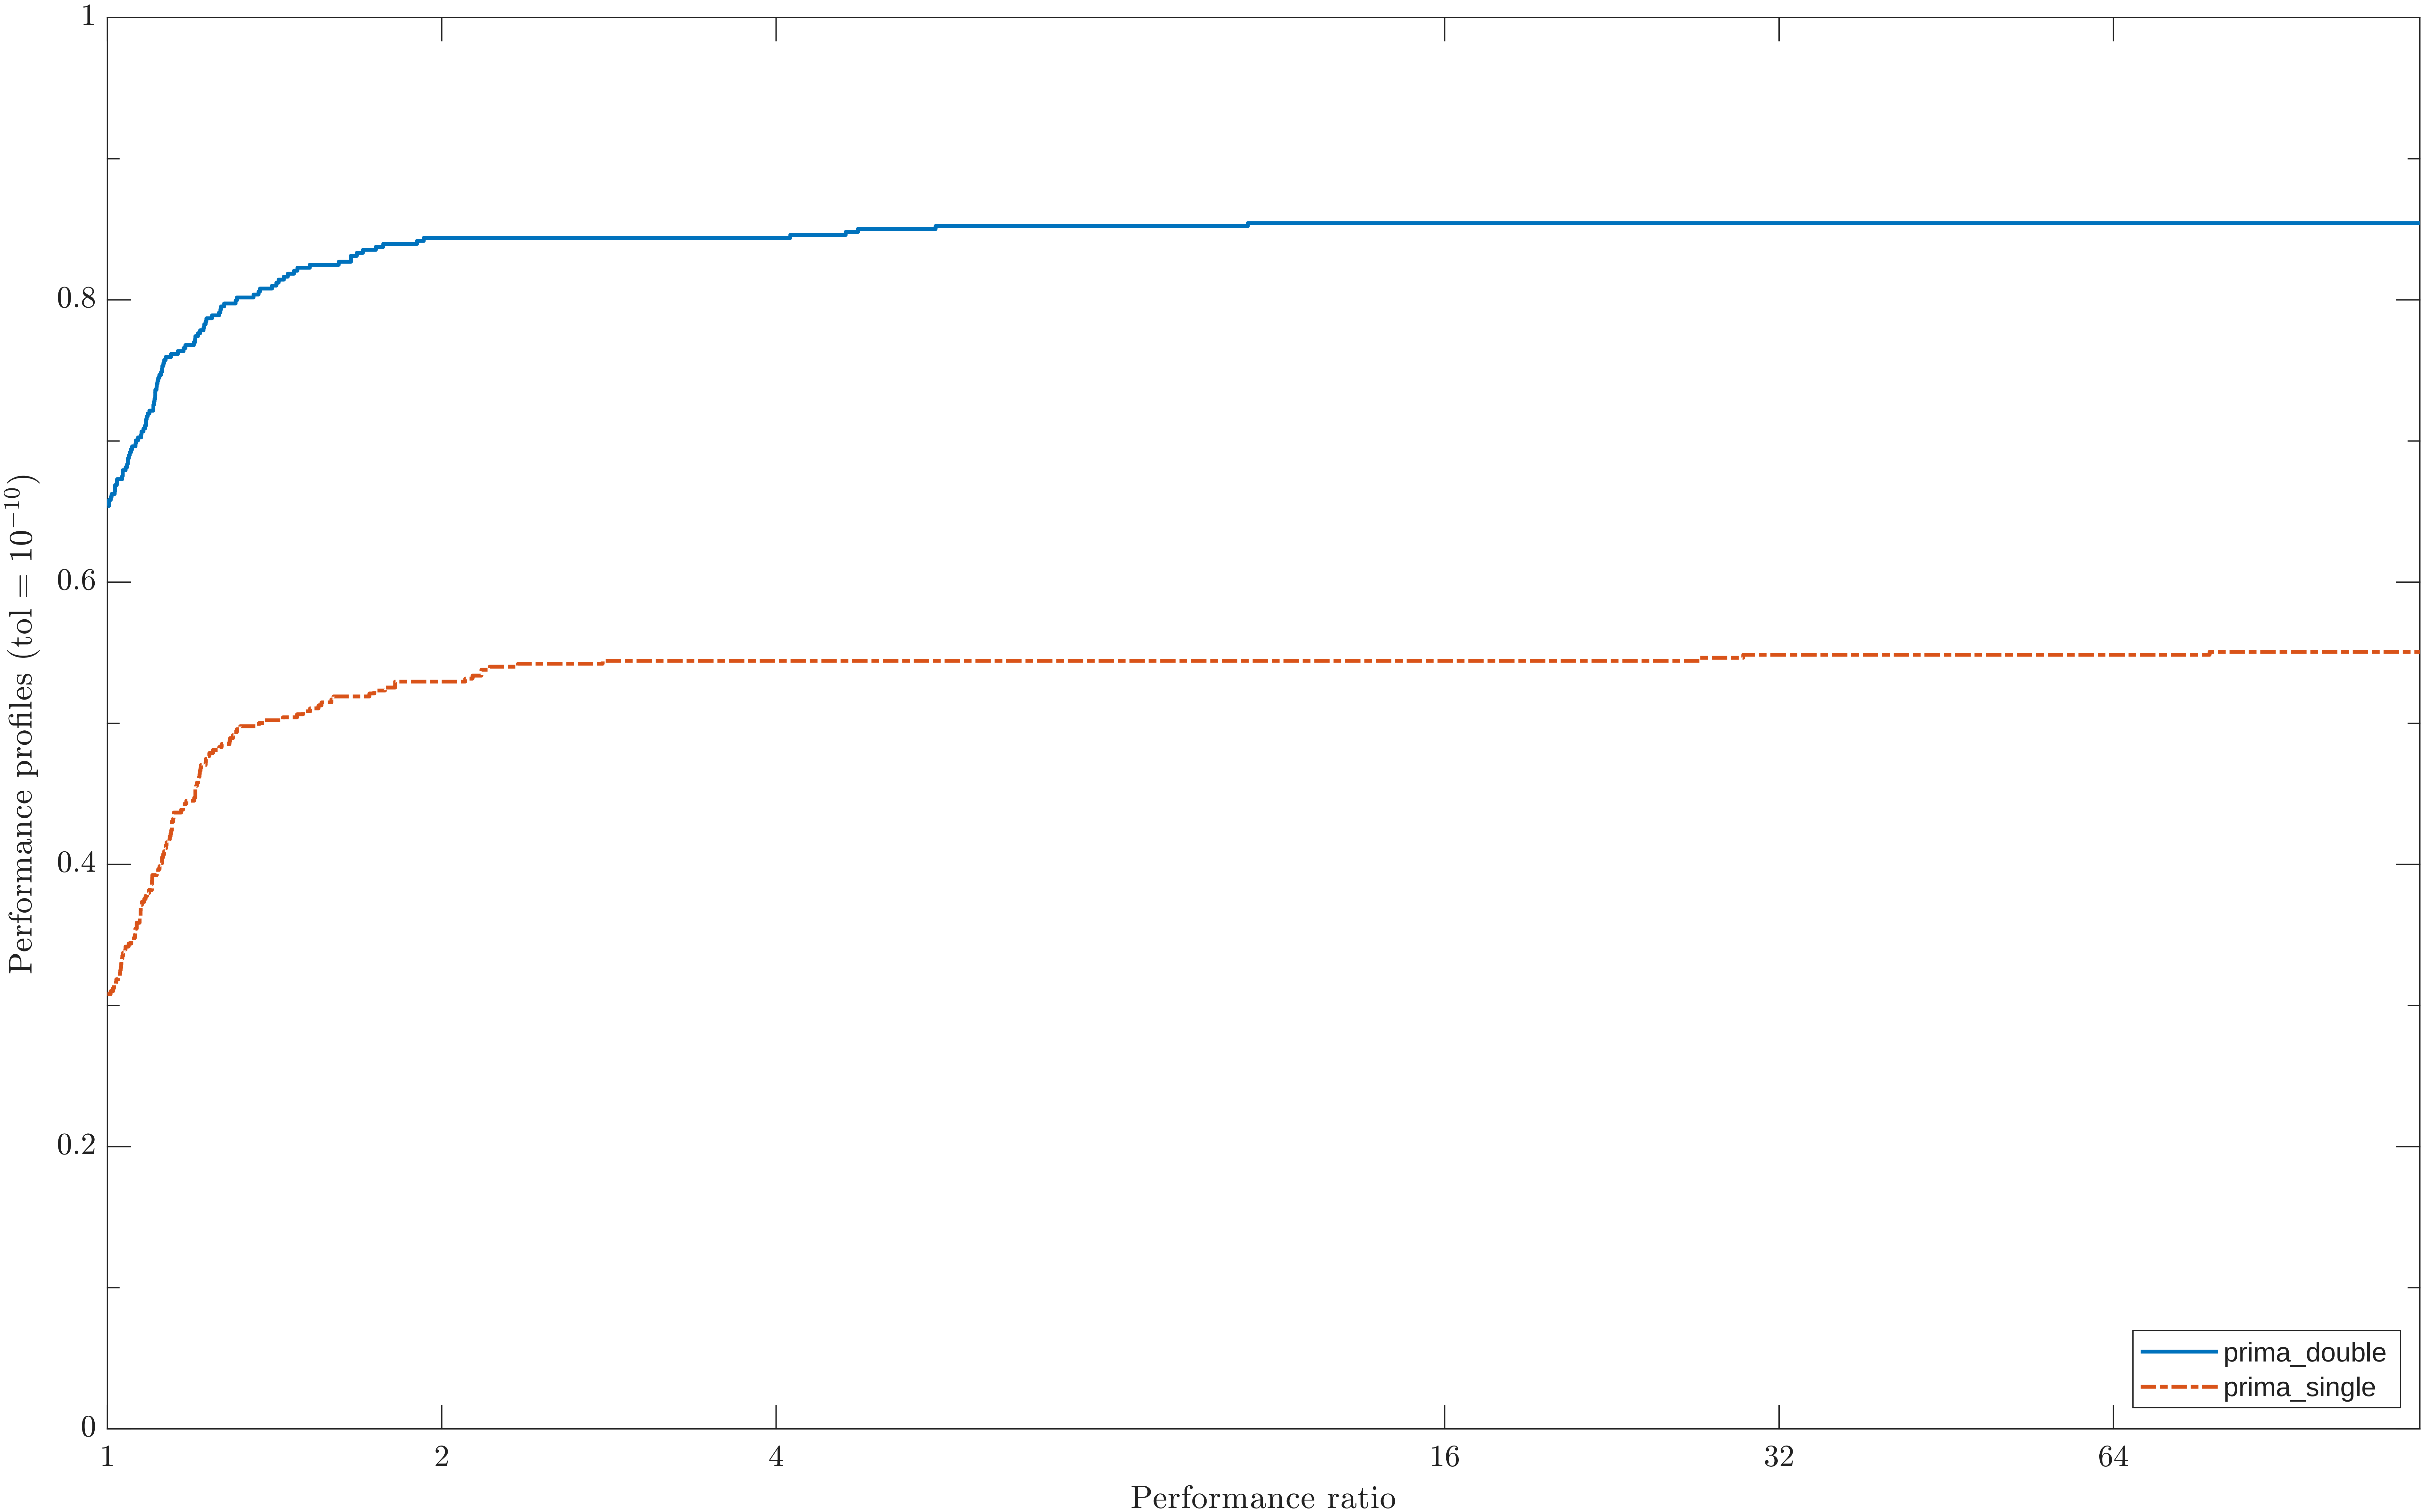
\includegraphics[width=0.75\textwidth]{figures/perf_out_plain_ds.png}
    \caption{Performance profiles for double and single precision on the plain problem set.}
    \label{fig:perf_out_plain_ds}
\end{figure}

\begin{figure}[H]
    \centering
    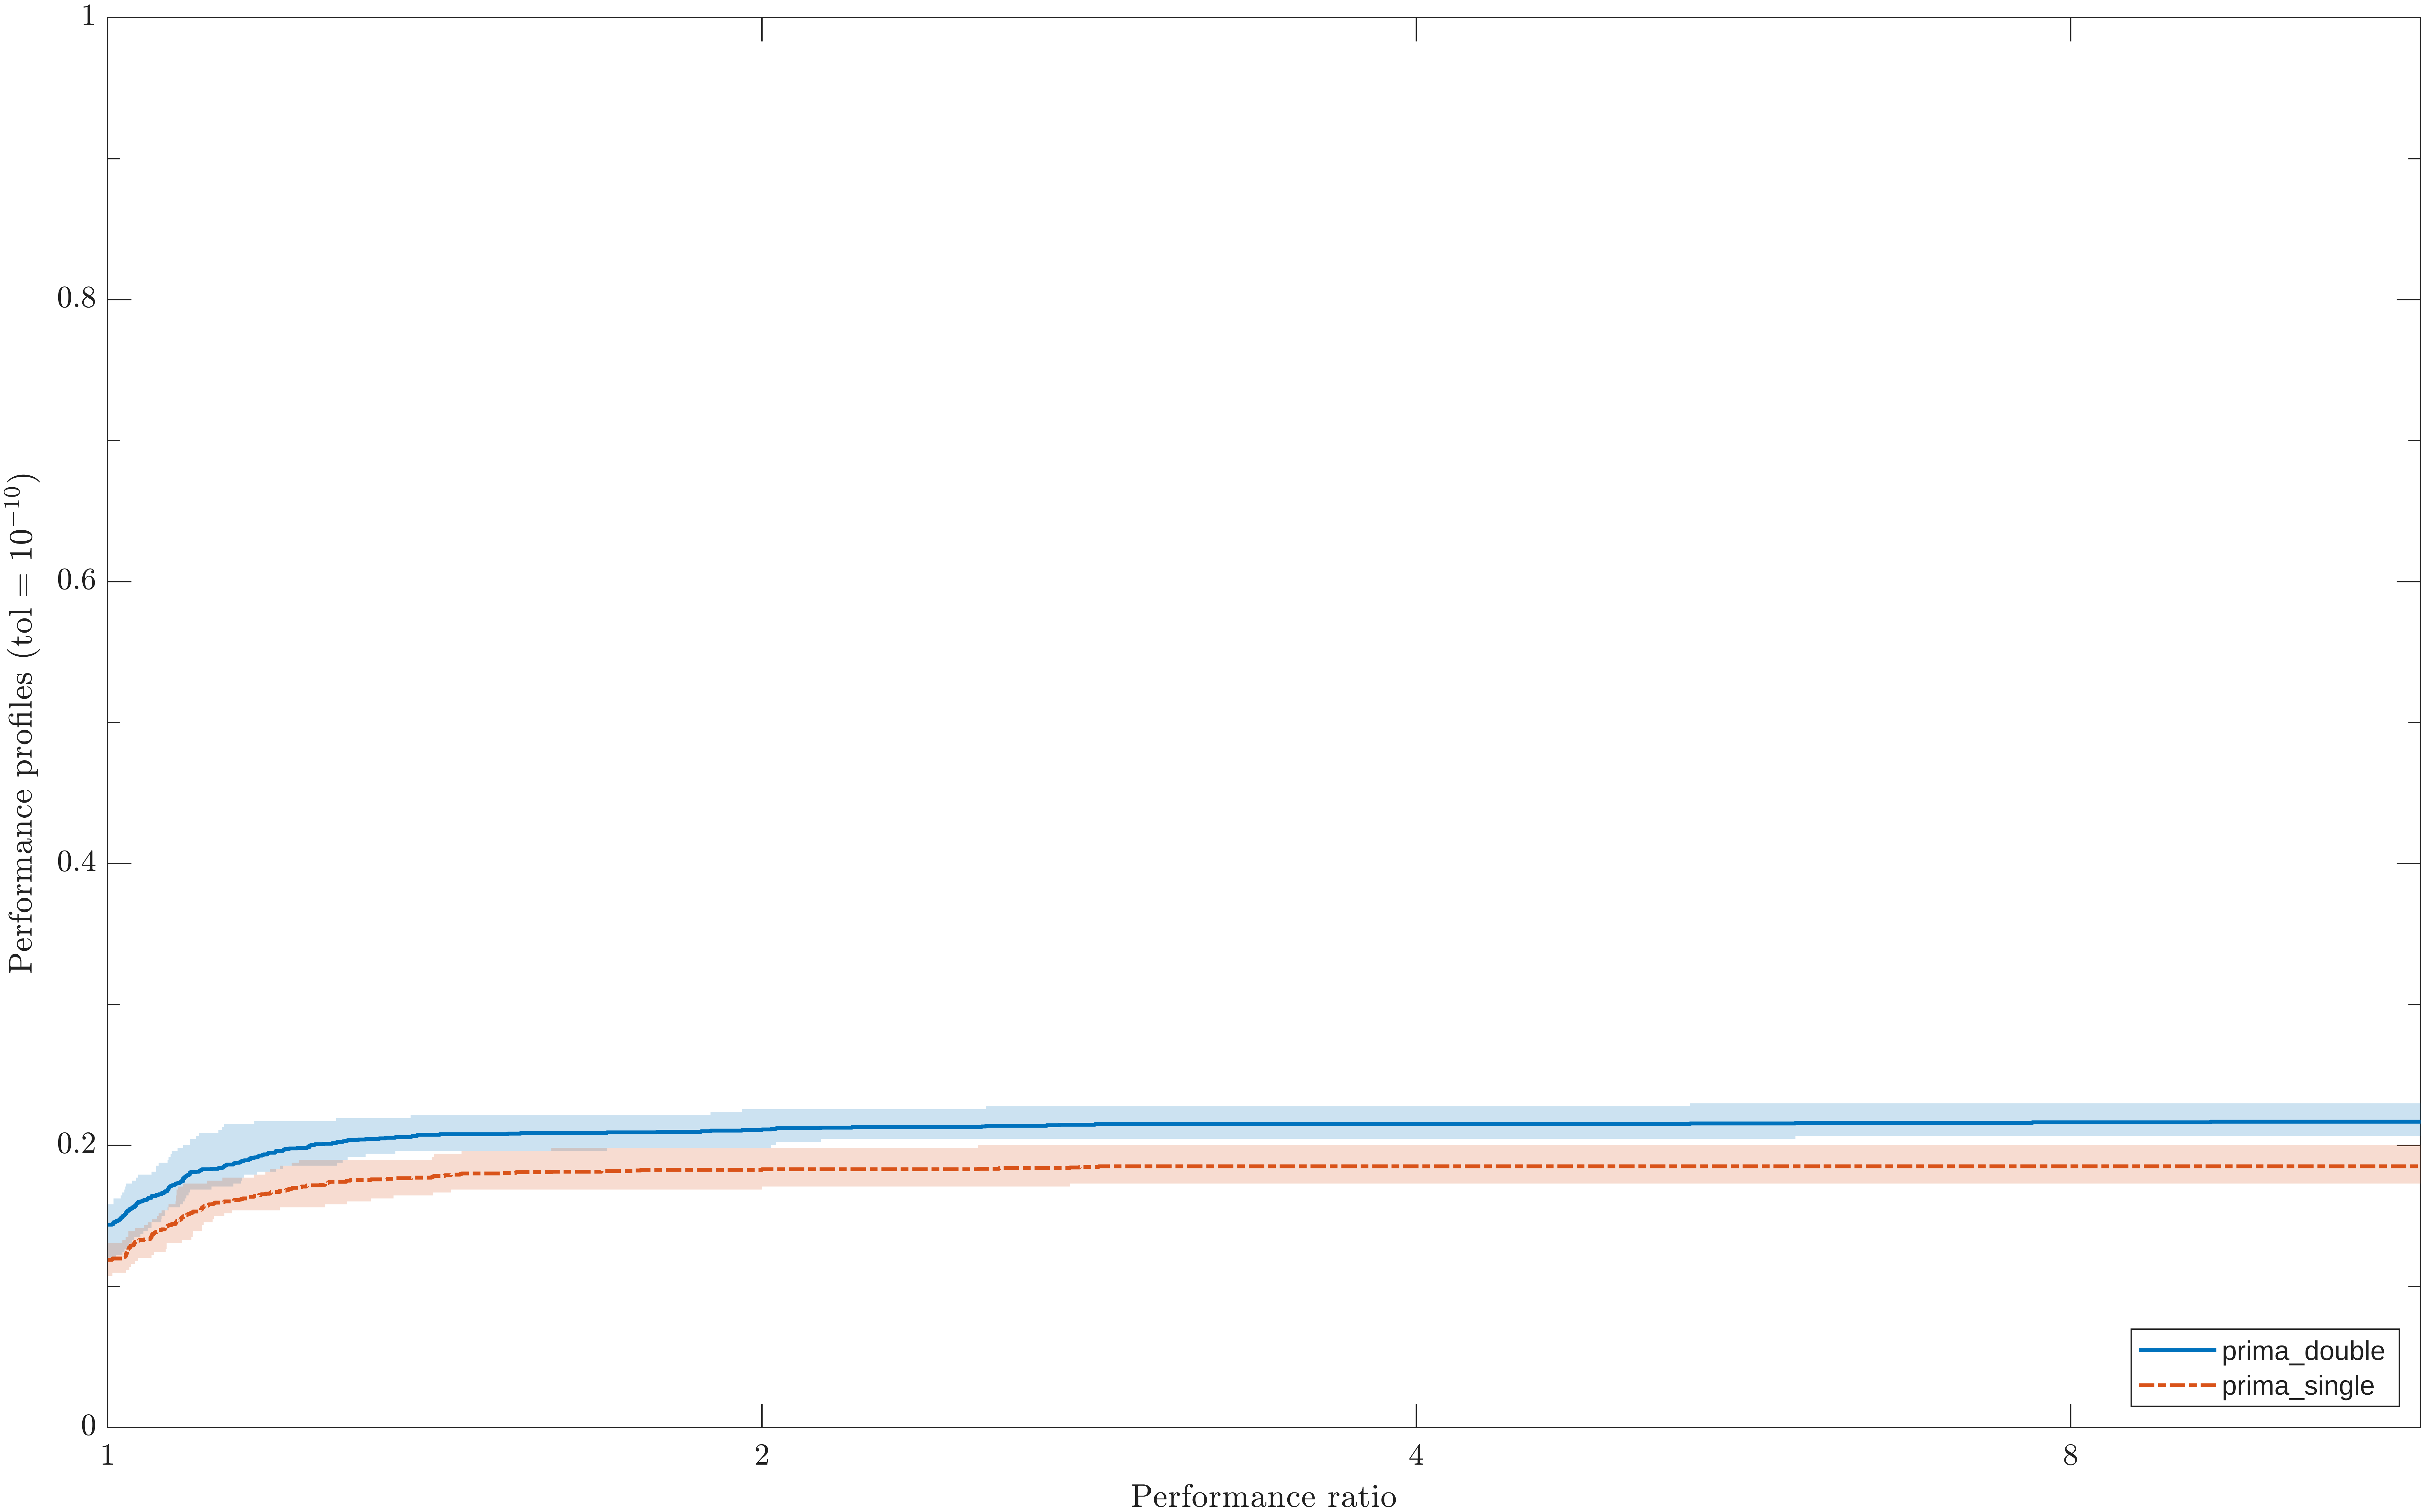
\includegraphics[width=0.75\textwidth]{figures/perf_out_noisy_ds.png}
    \caption{Performance profiles for double and single precision on the noisy problem set.}
    \label{fig:perf_out_noisy_ds}
\end{figure}

\begin{figure}[H]
    \centering
    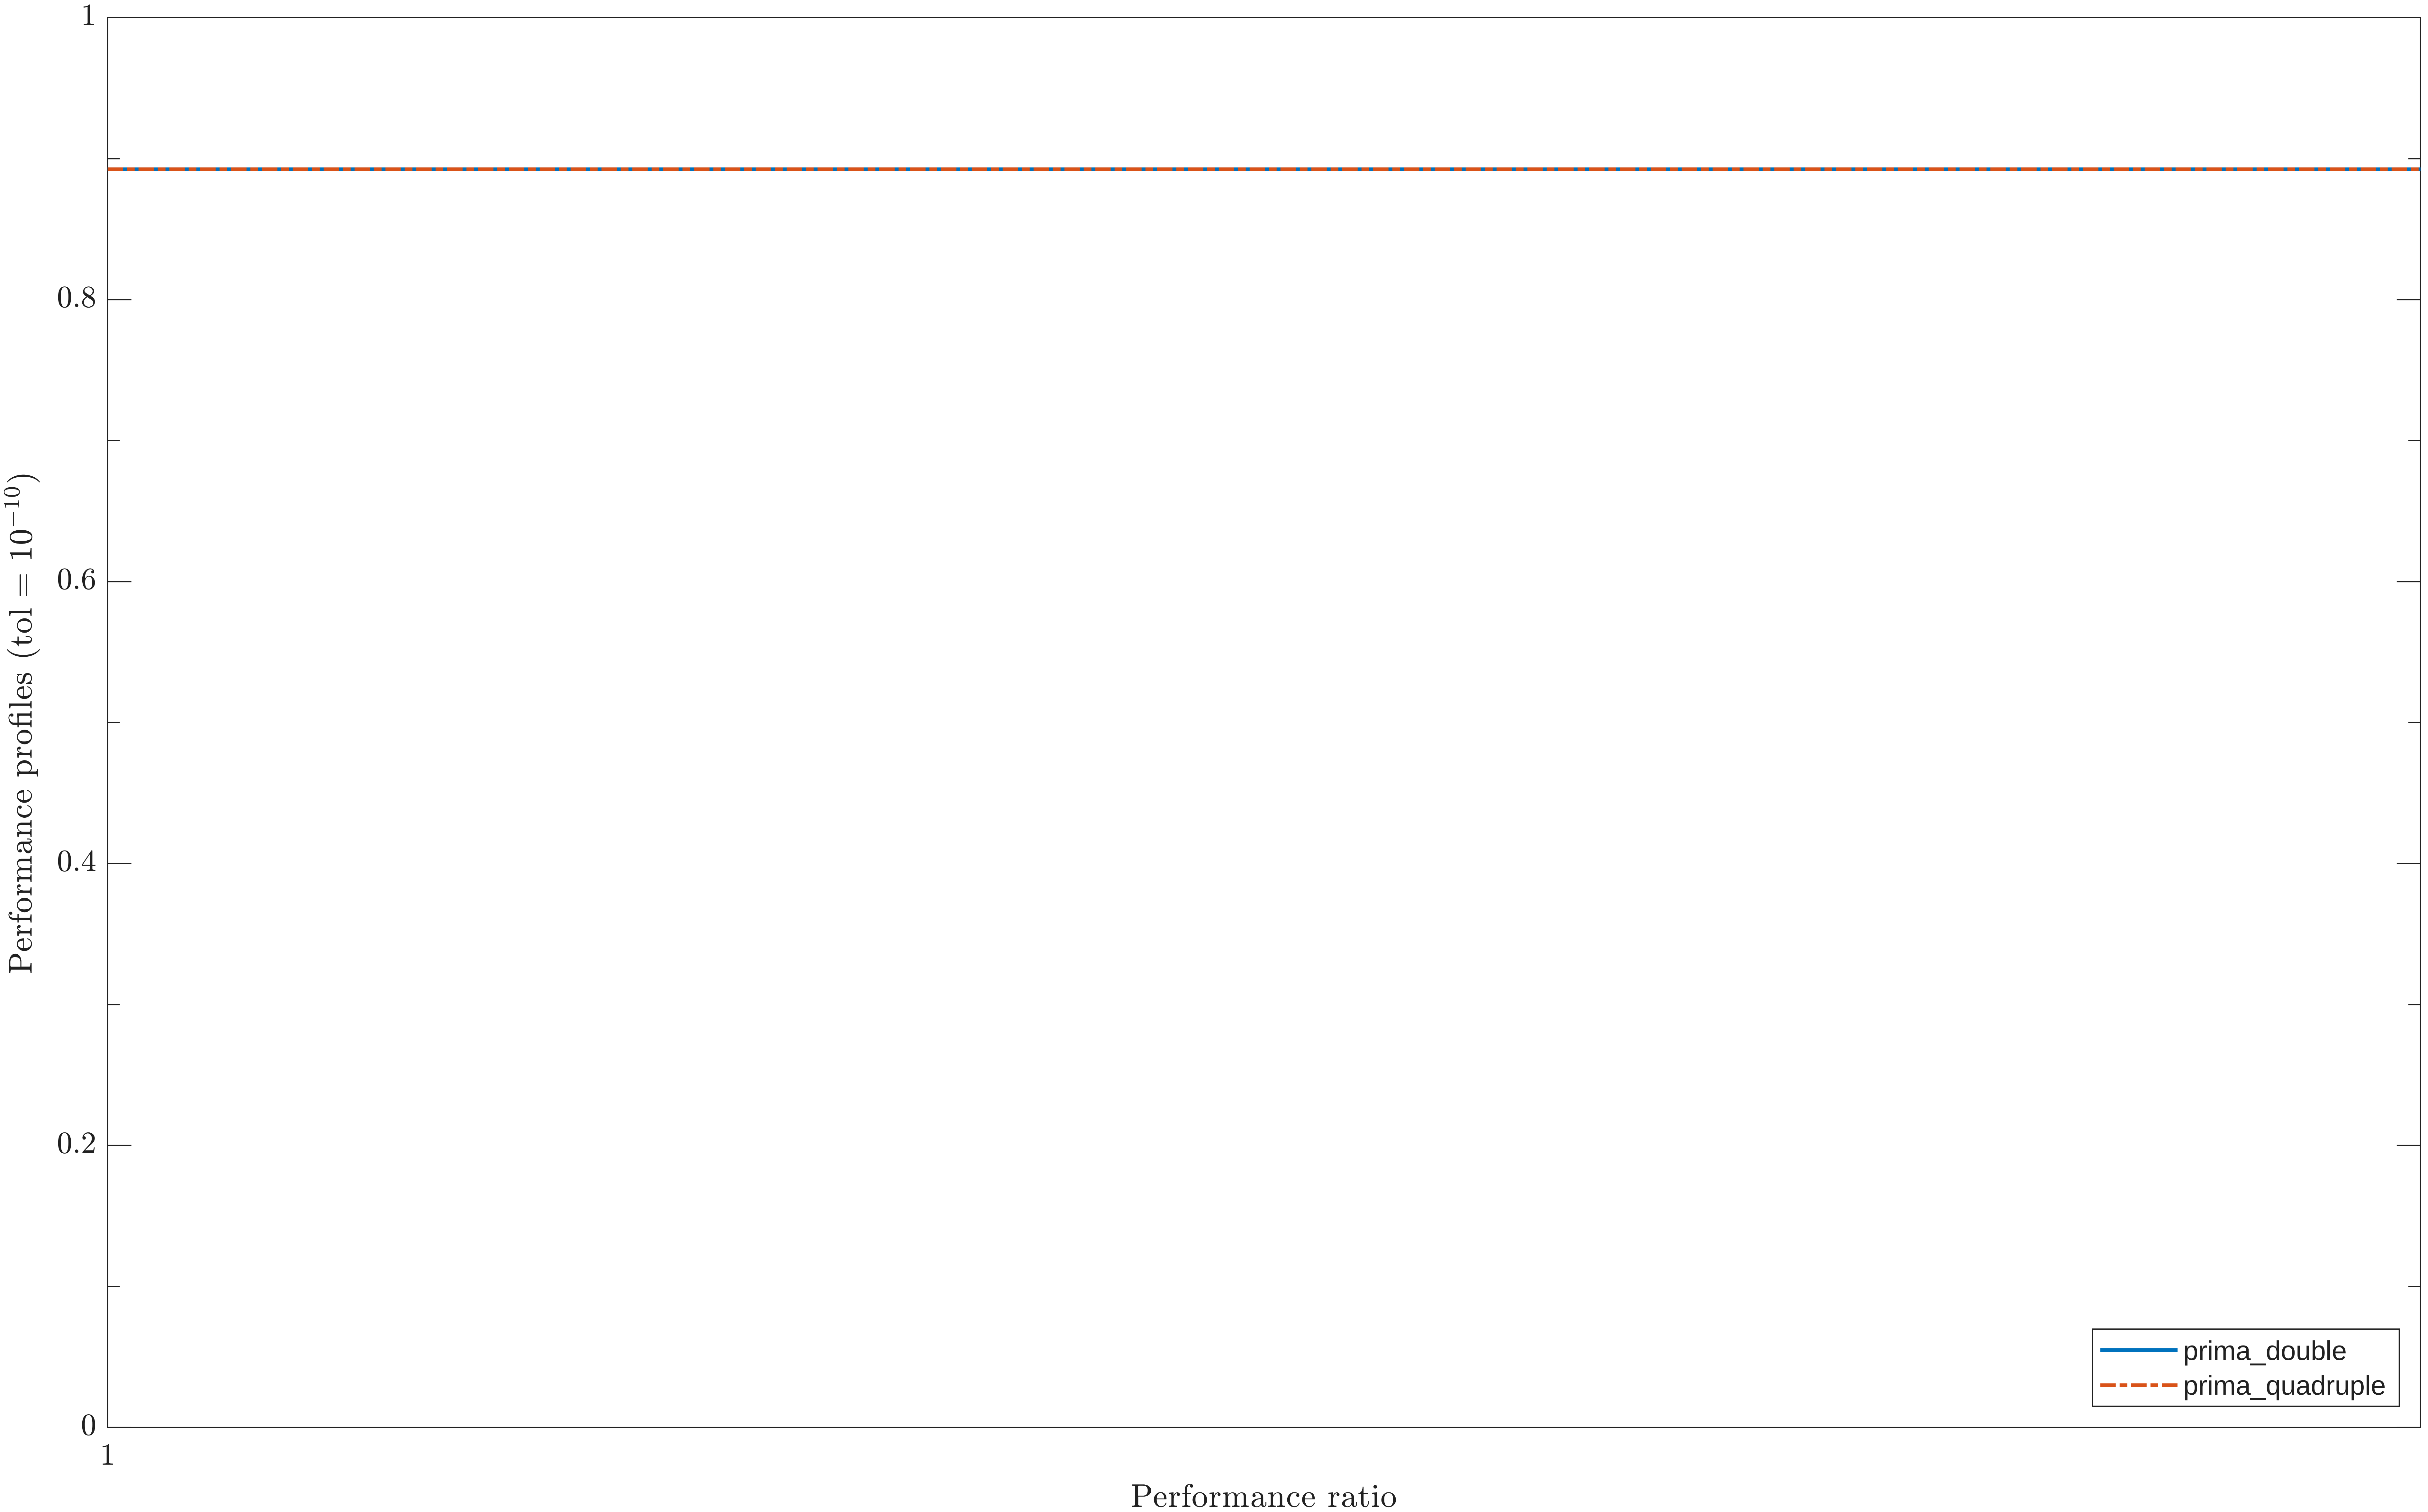
\includegraphics[width=0.75\textwidth]{figures/perf_out_plain_dq.png}
    \caption{Performance profiles for double and quadruple precision on the plain problem set.}
    \label{fig:perf_out_plain_dq}
\end{figure}

\begin{figure}[H]
    \centering
    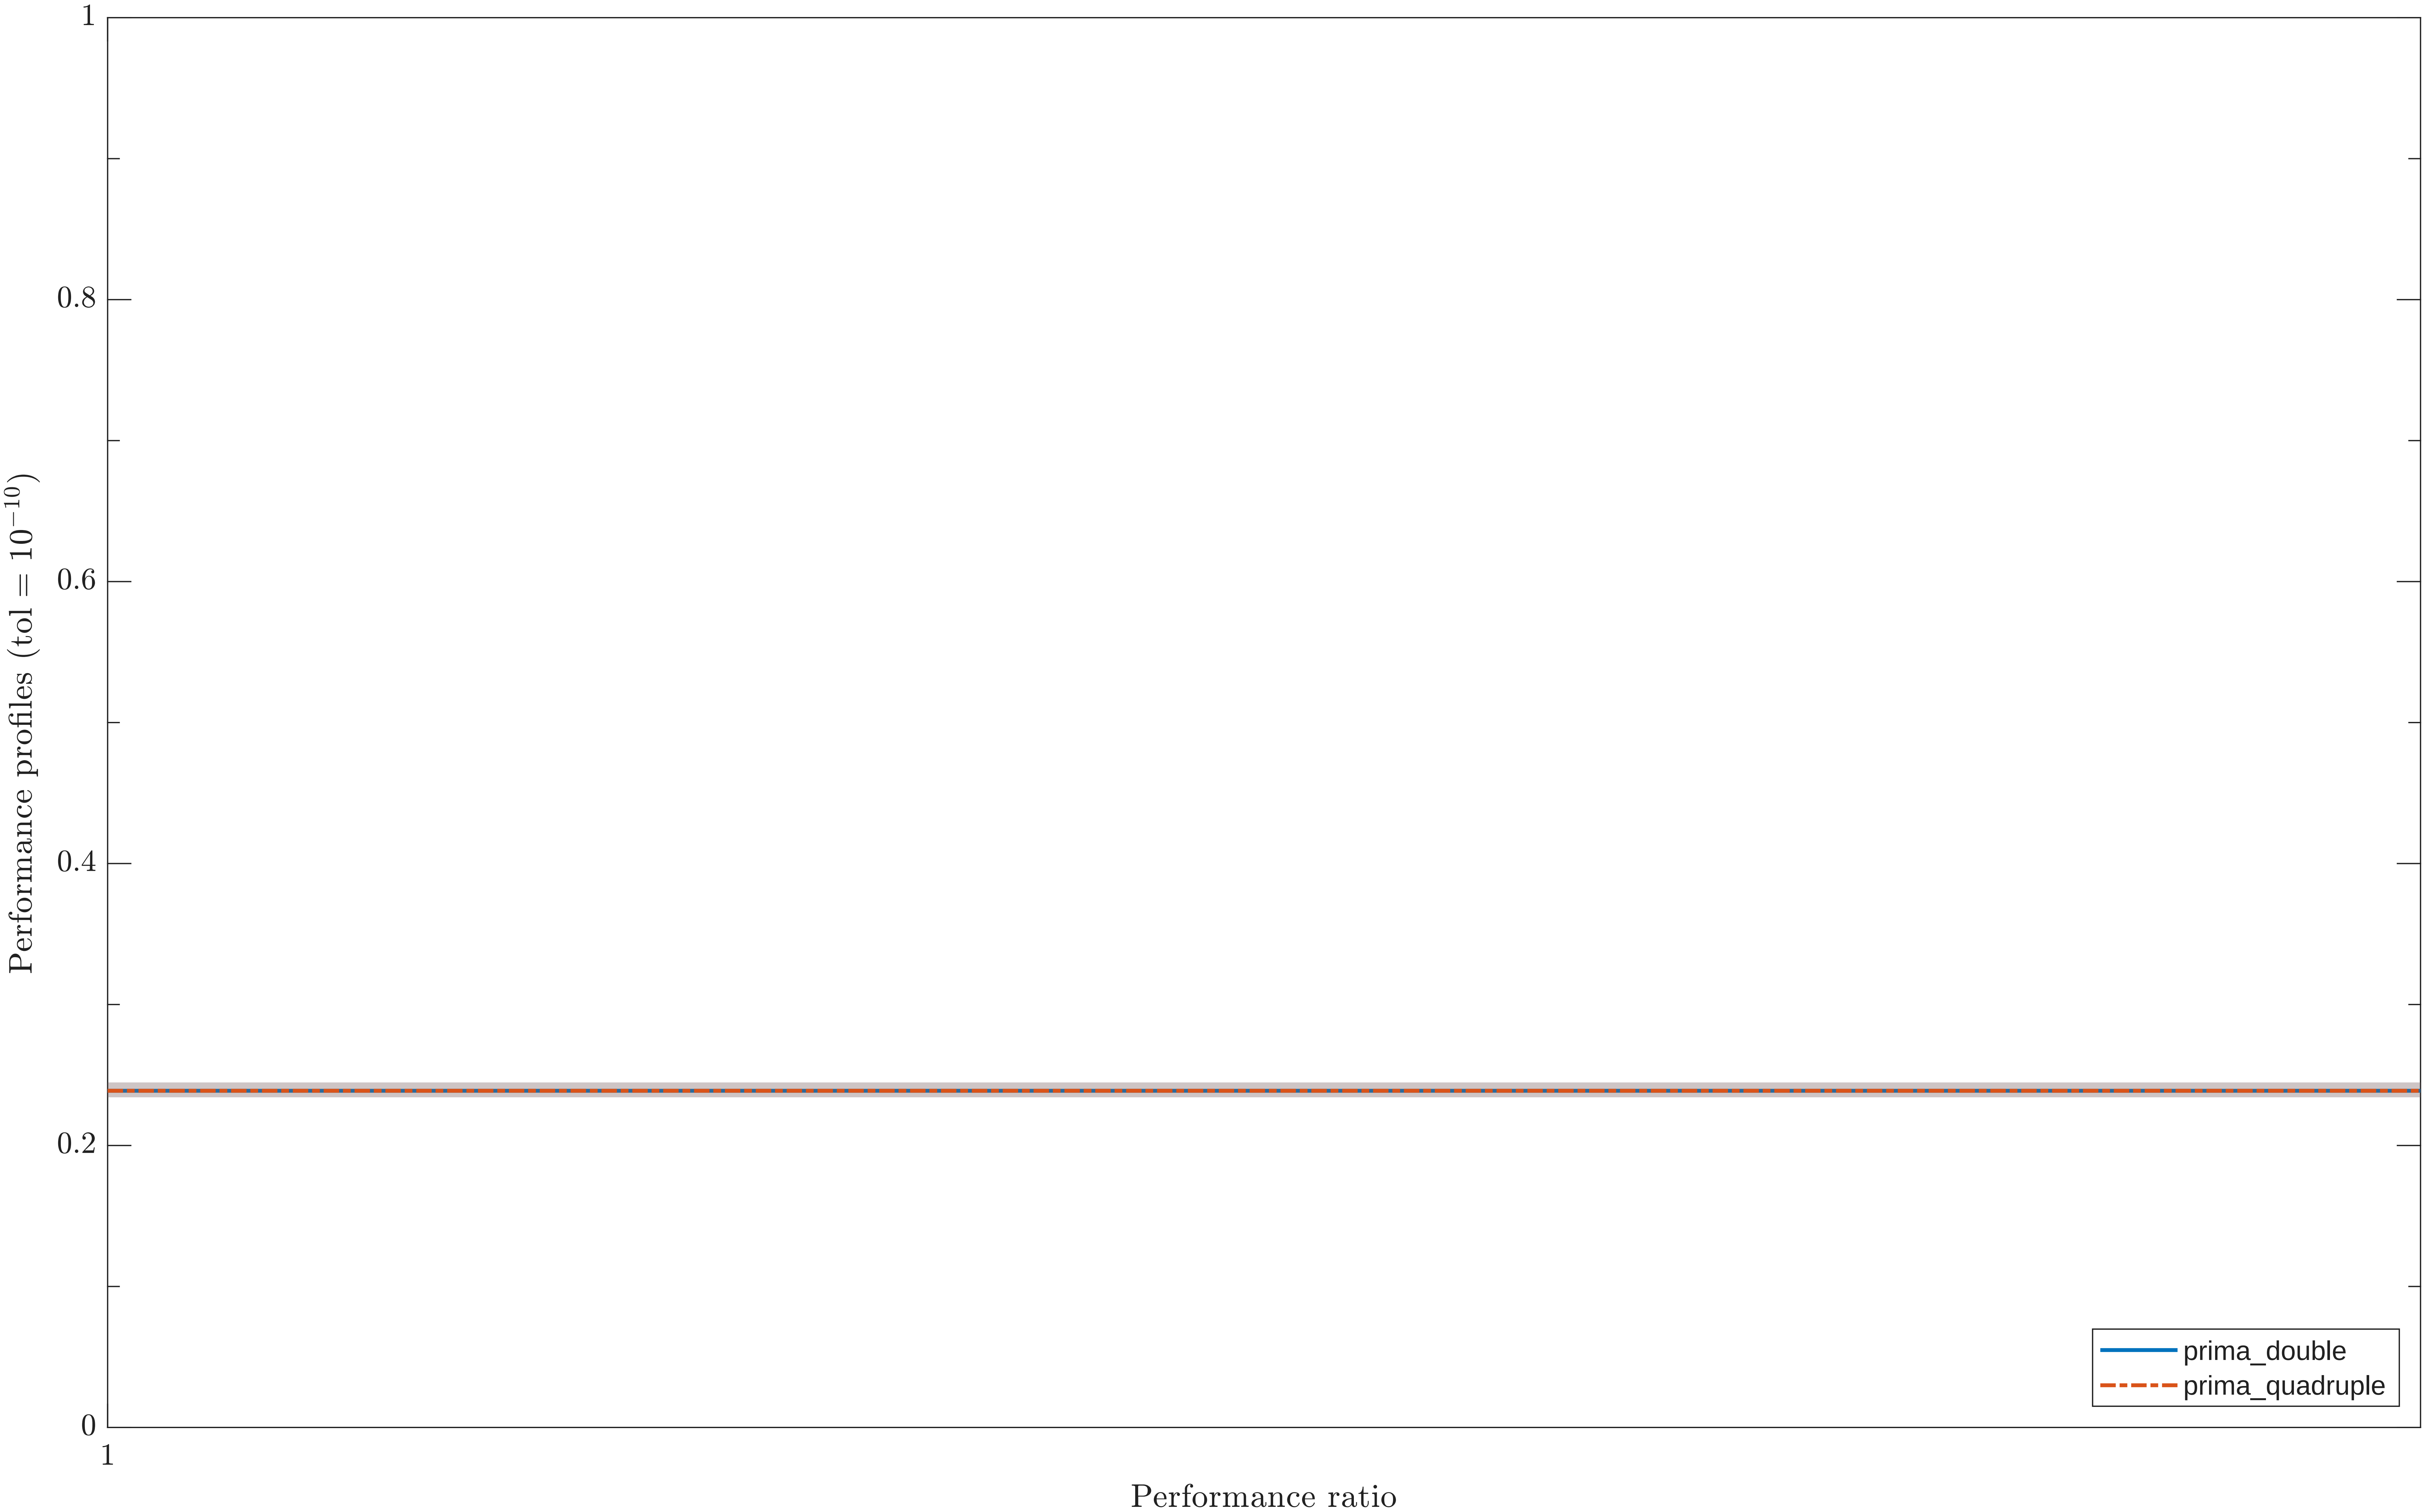
\includegraphics[width=0.75\textwidth]{figures/perf_out_noisy_dq.png}
    \caption{Performance profiles for double and quadruple precision on the noisy problem set.}
    \label{fig:perf_out_noisy_dq}
\end{figure}

Figure~\ref{fig:perf_out_plain_ds} and Table~\ref{tab:ds_plain} compare
the double-precision and single-precision cases on the plain and noisy
problem sets. In both settings, double precision achieves a higher score
and a superior performance profile, with the advantage being particularly
evident in the noise‑free case. When Gaussian noise is introduced,
the gap between the two solvers narrows, but double precision remains
the better-performing option.

In contrast, the double-precision and quadruple-precision cases show no
meaningful difference. Their scores are identical, and their performance
profiles overlap almost completely across all tolerances. This holds for
both the plain and the noisy features, suggesting that double precision
already provides sufficient numerical resolution for the tested problems.

All profiles shown in this section correspond to the strictest tolerance
($10^{-10}$). This tolerance was chosen because it magnifies the
differences between solvers that would otherwise appear indistinguishable
under looser convergence criteria. We can always notice that each
precision degrades significantly in the noisy setting.

% --- Data Profiles ---
\begin{figure}[H]
    \centering
    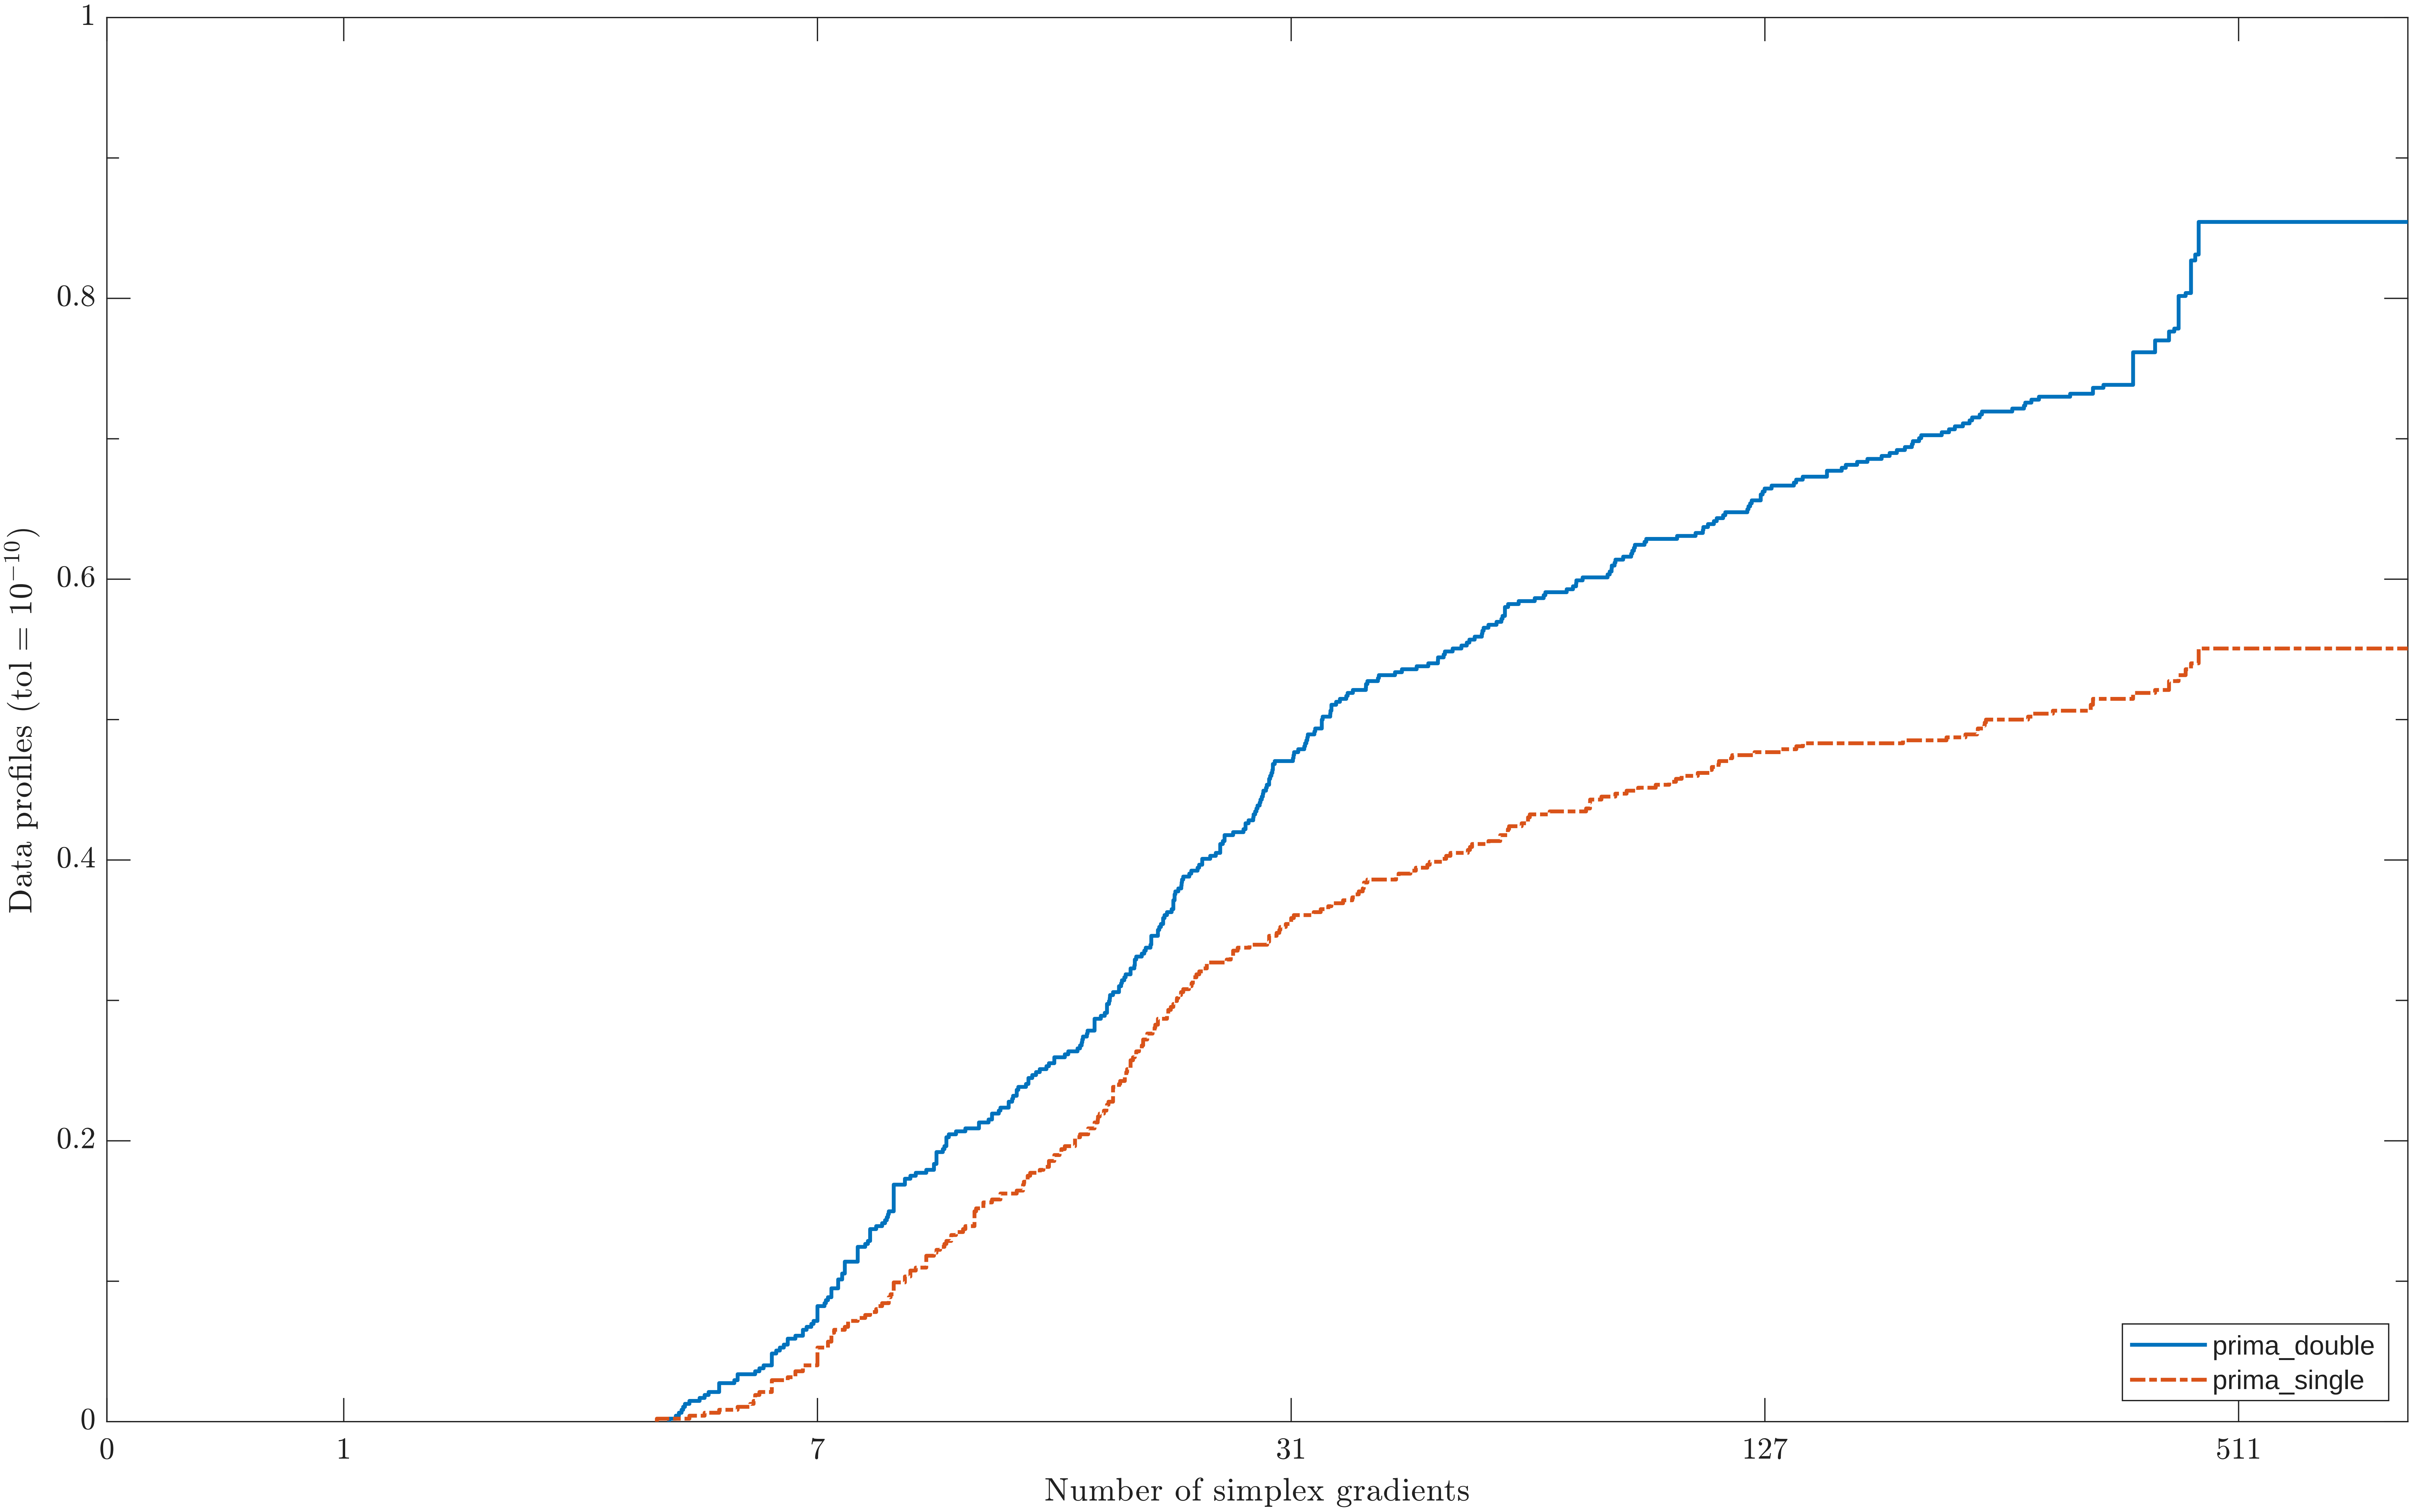
\includegraphics[width=0.75\textwidth]{figures/data_out_10_plain_ds.png}
    \caption{Data profiles for double and single precision on the plain problem set at tolerance $10^{-10}$.}
    \label{fig:data_out_plain_ds}
\end{figure}

\begin{figure}[H]
    \centering
    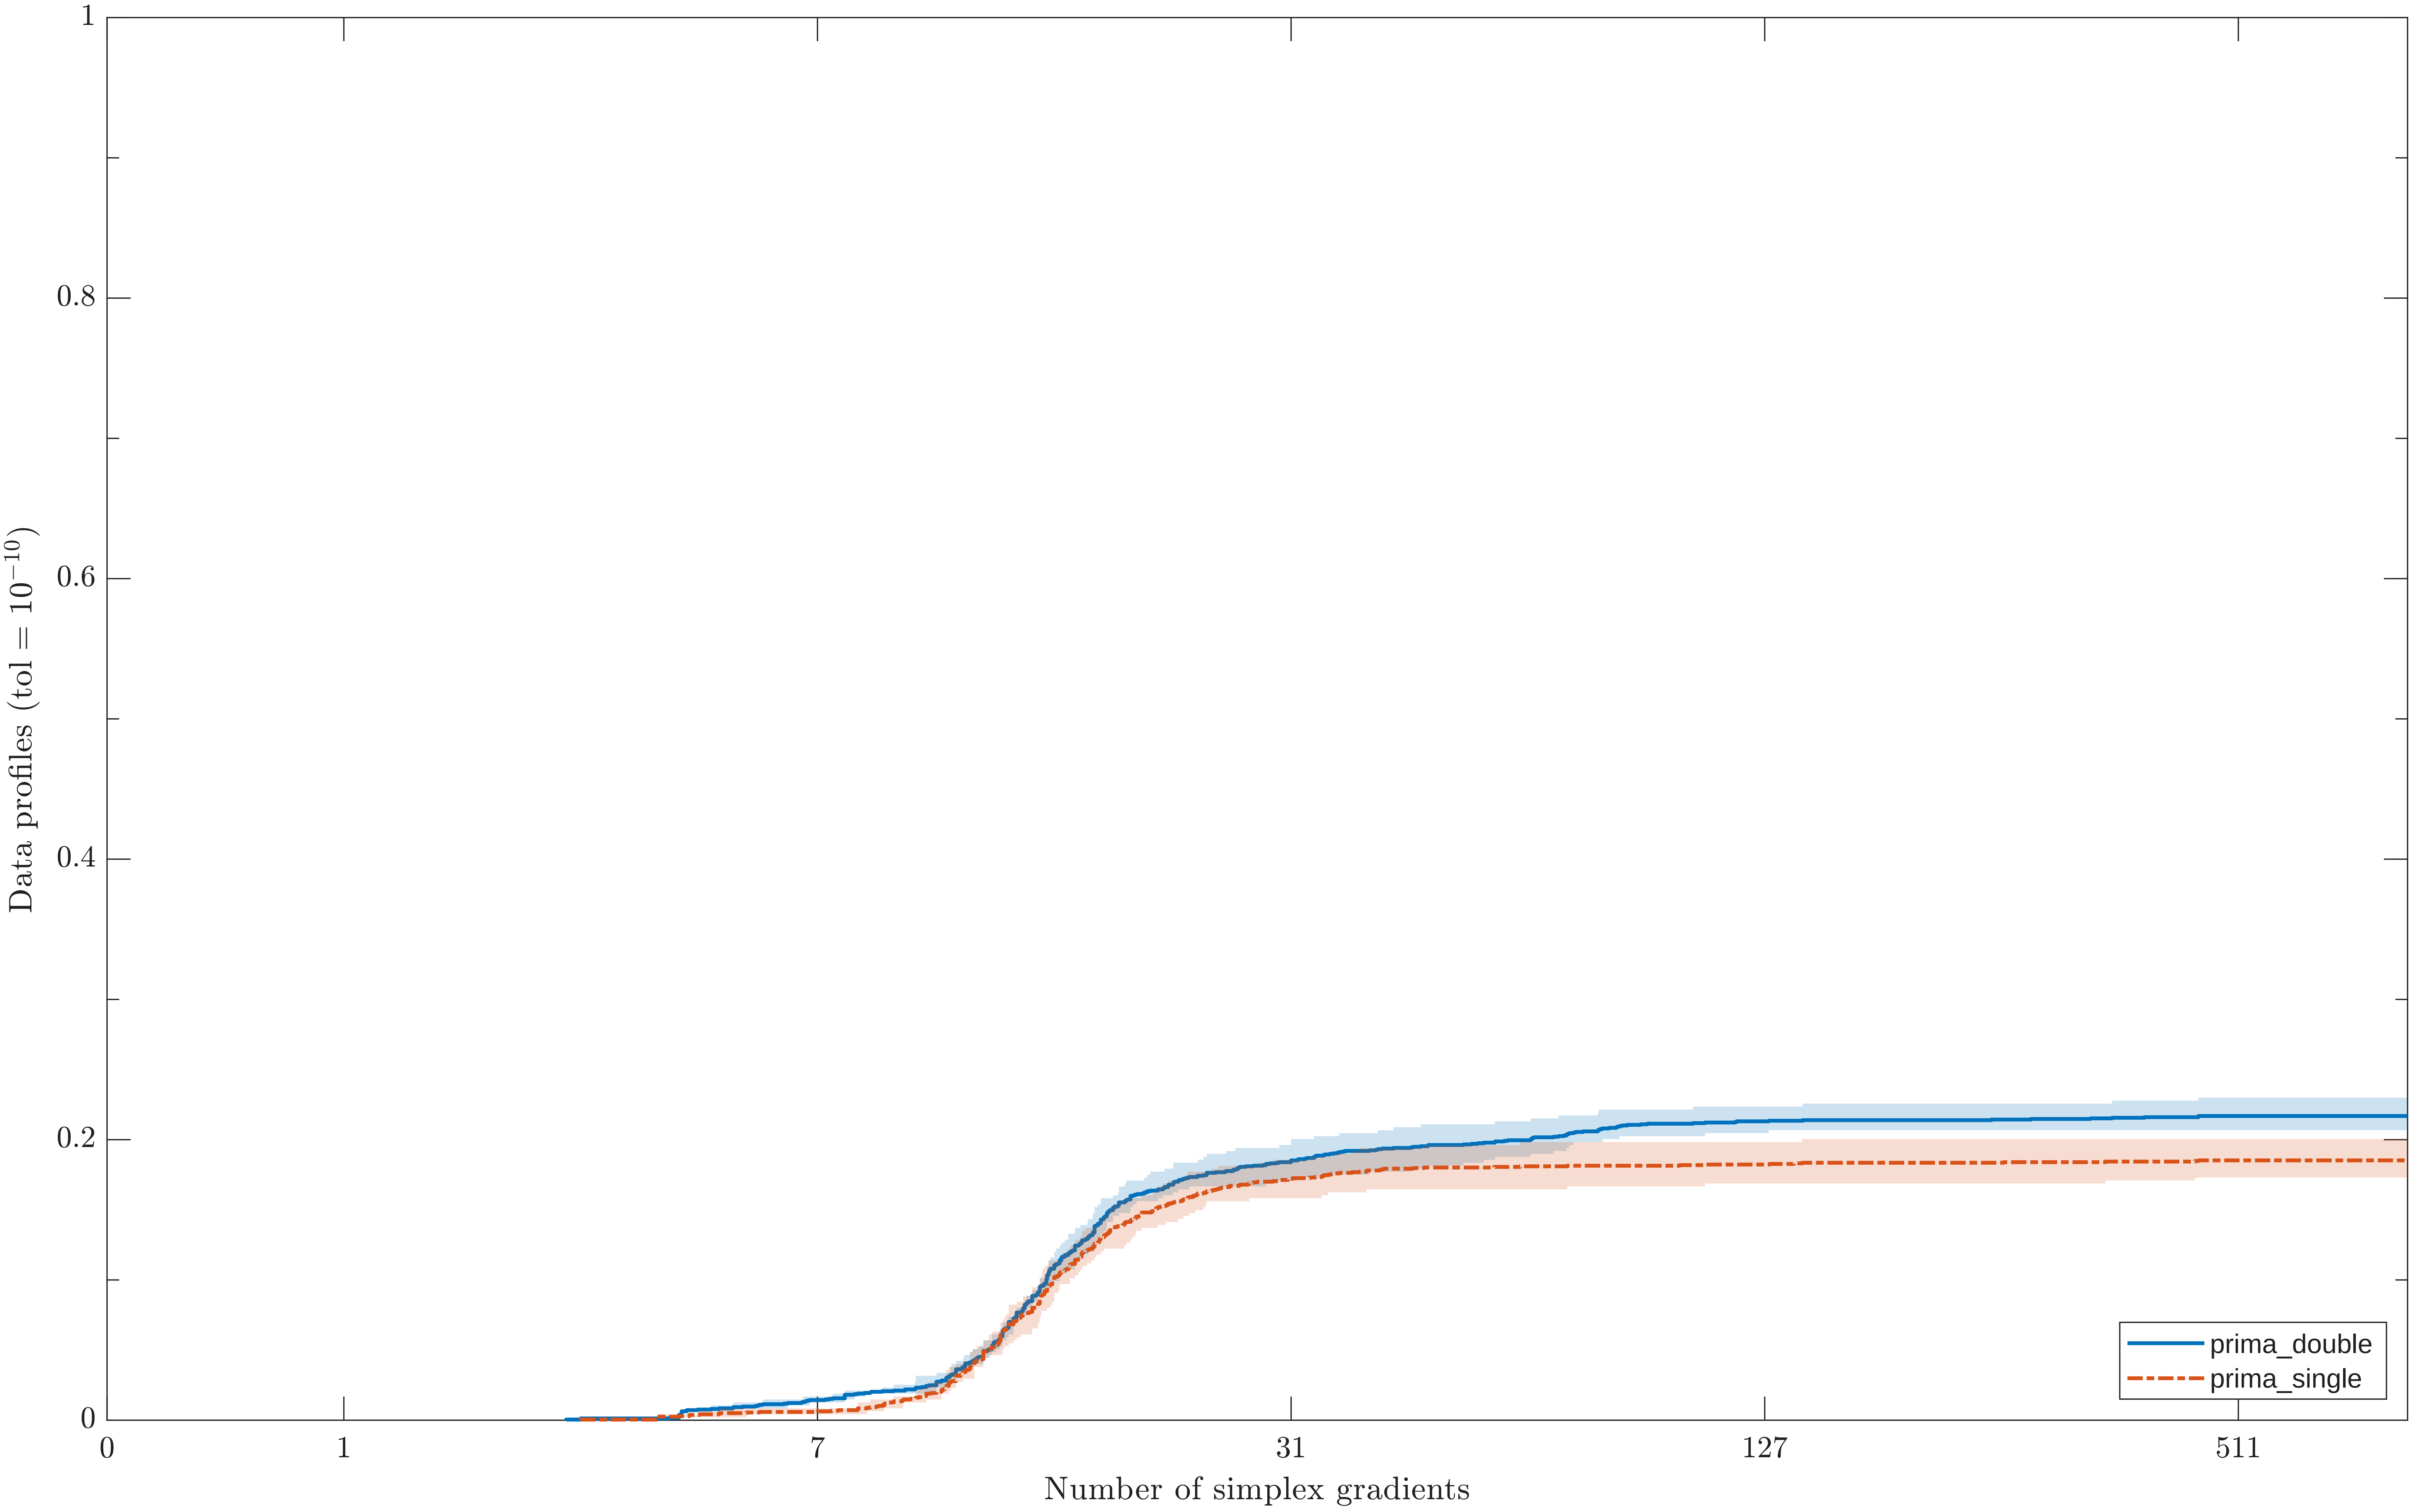
\includegraphics[width=0.75\textwidth]{figures/data_out_noisy_ds.png}
    \caption{Data profiles for double and single precision on the noisy problem set.}
    \label{fig:data_out_noisy_ds}
\end{figure}

% --- Log-Ratio Profiles ---
\begin{figure}[H]
    \centering
    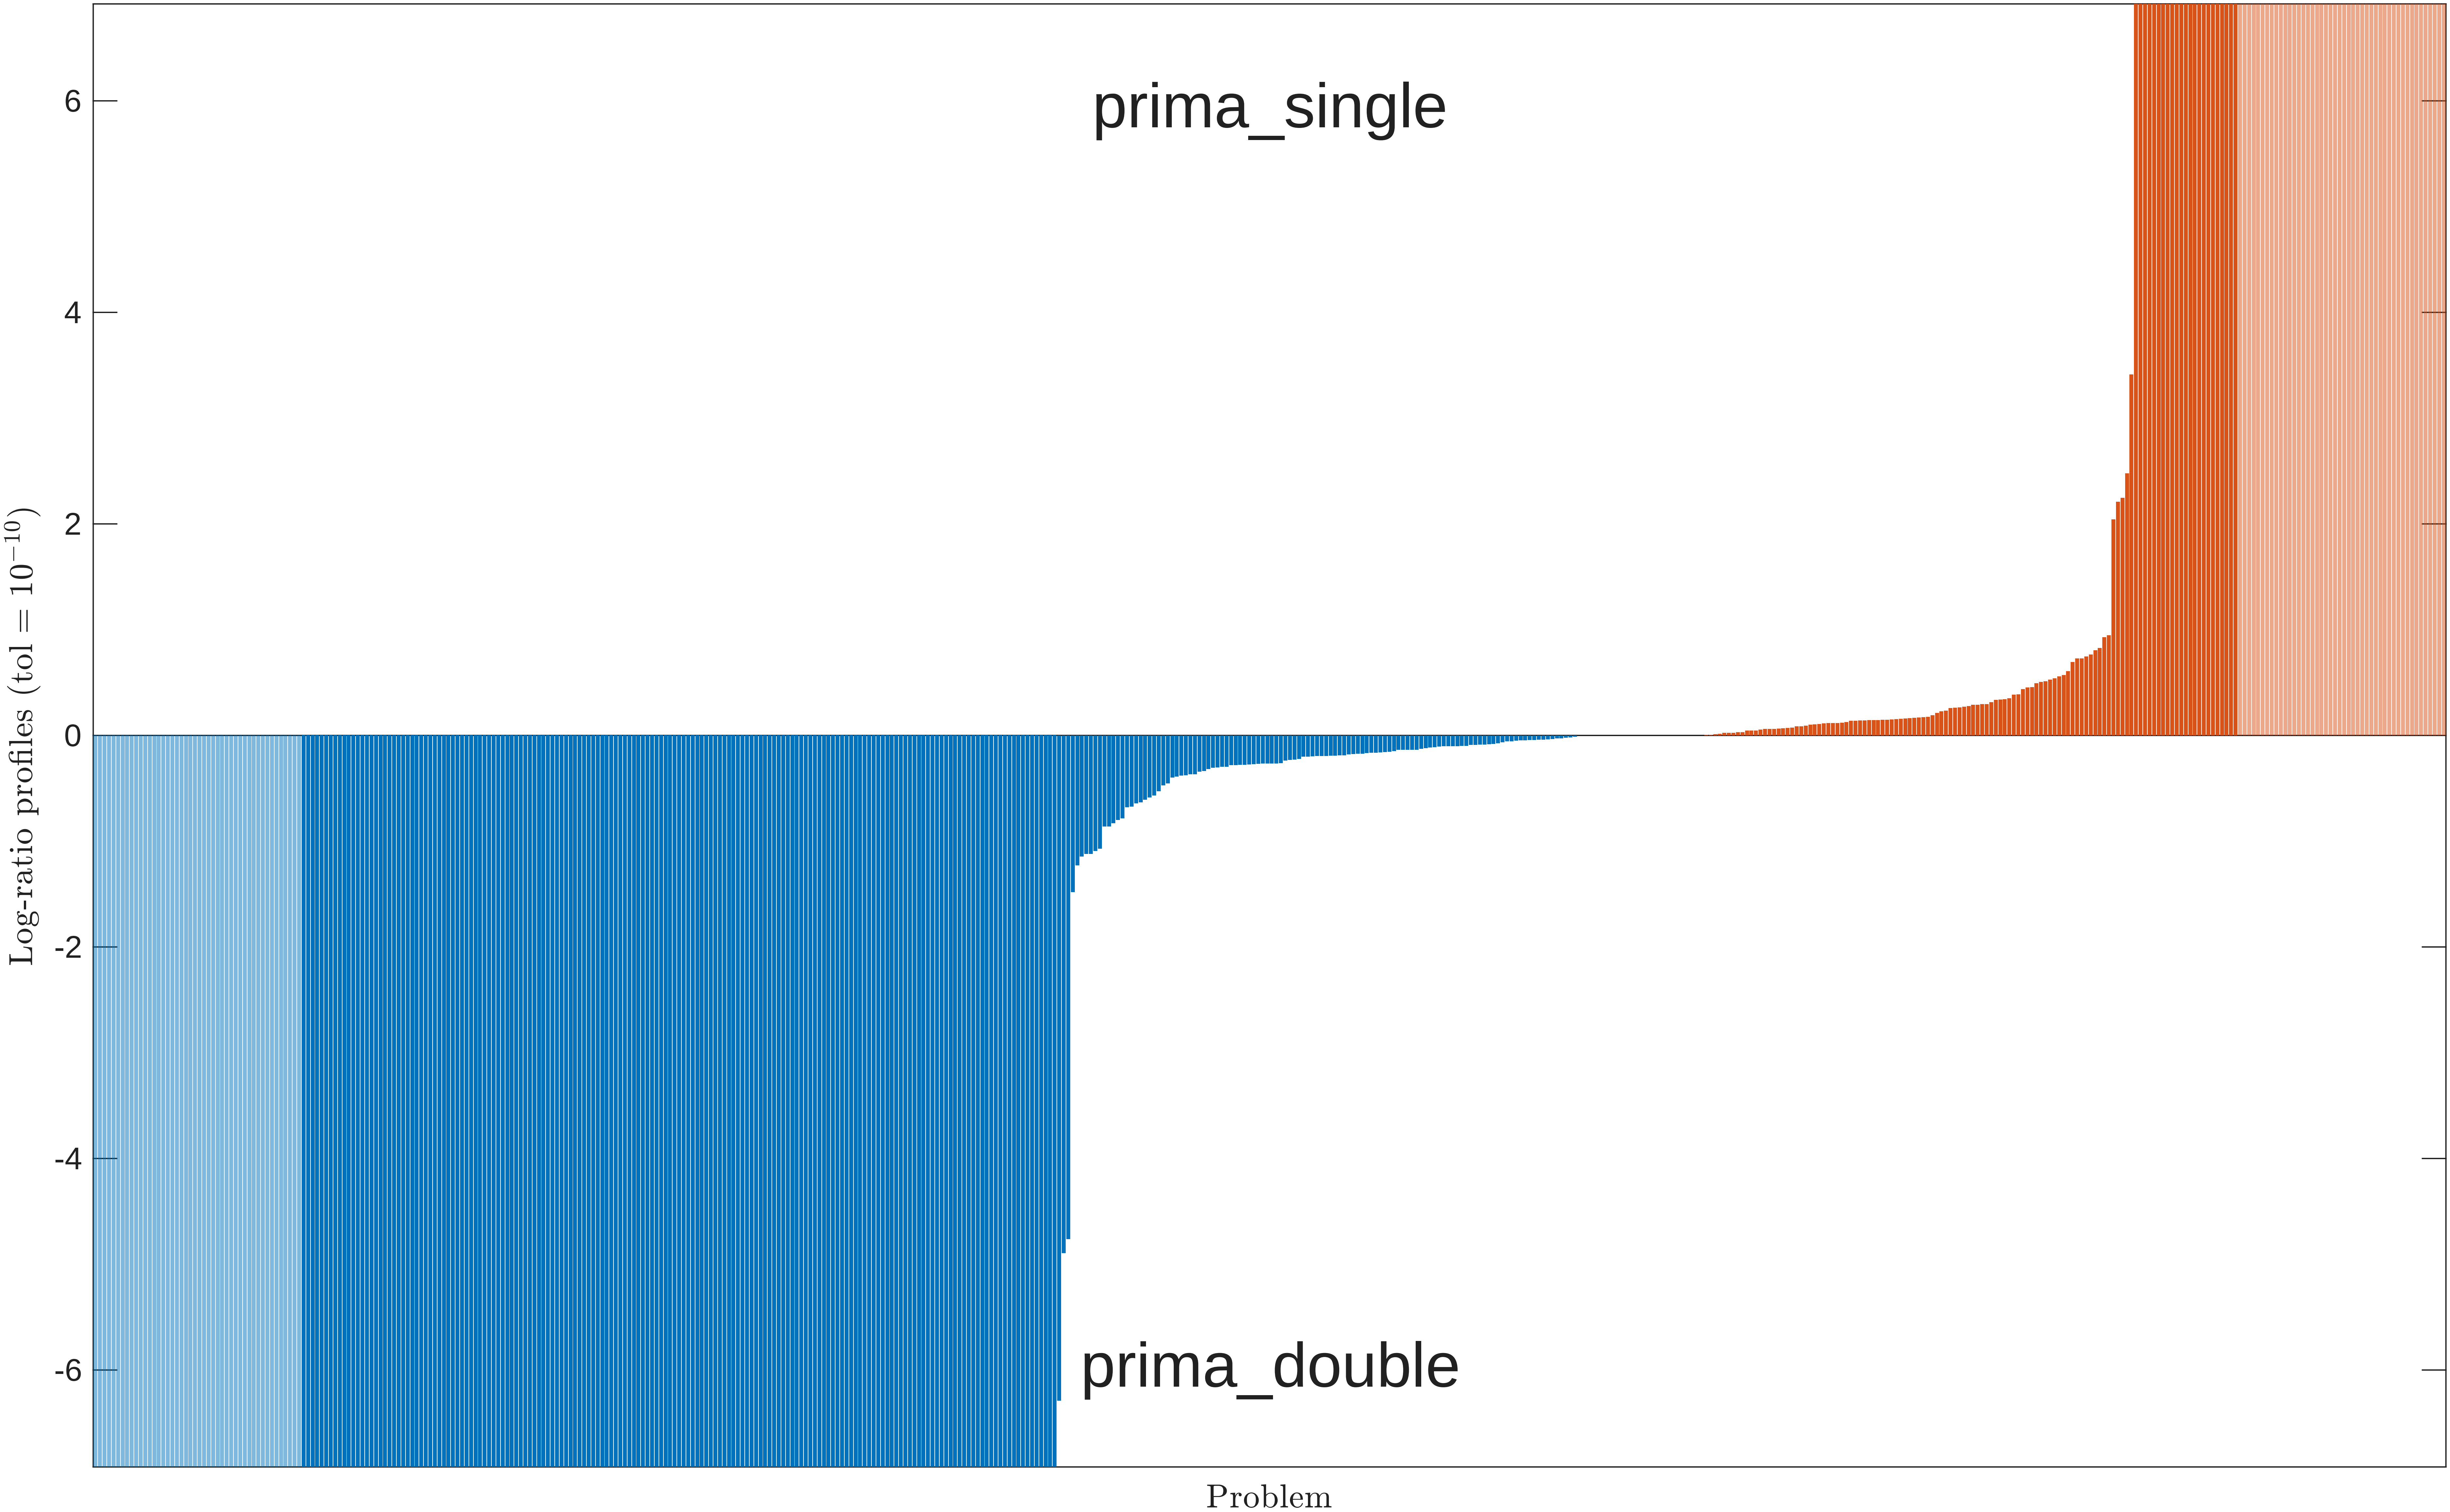
\includegraphics[width=0.75\textwidth]{figures/ration_plain_ds.png}
    \caption{Log-ratio profiles for double and single precision on the plain problem set.}
    \label{fig:log_ratio_plain_ds}
\end{figure}

\begin{figure}[H]
    \centering
    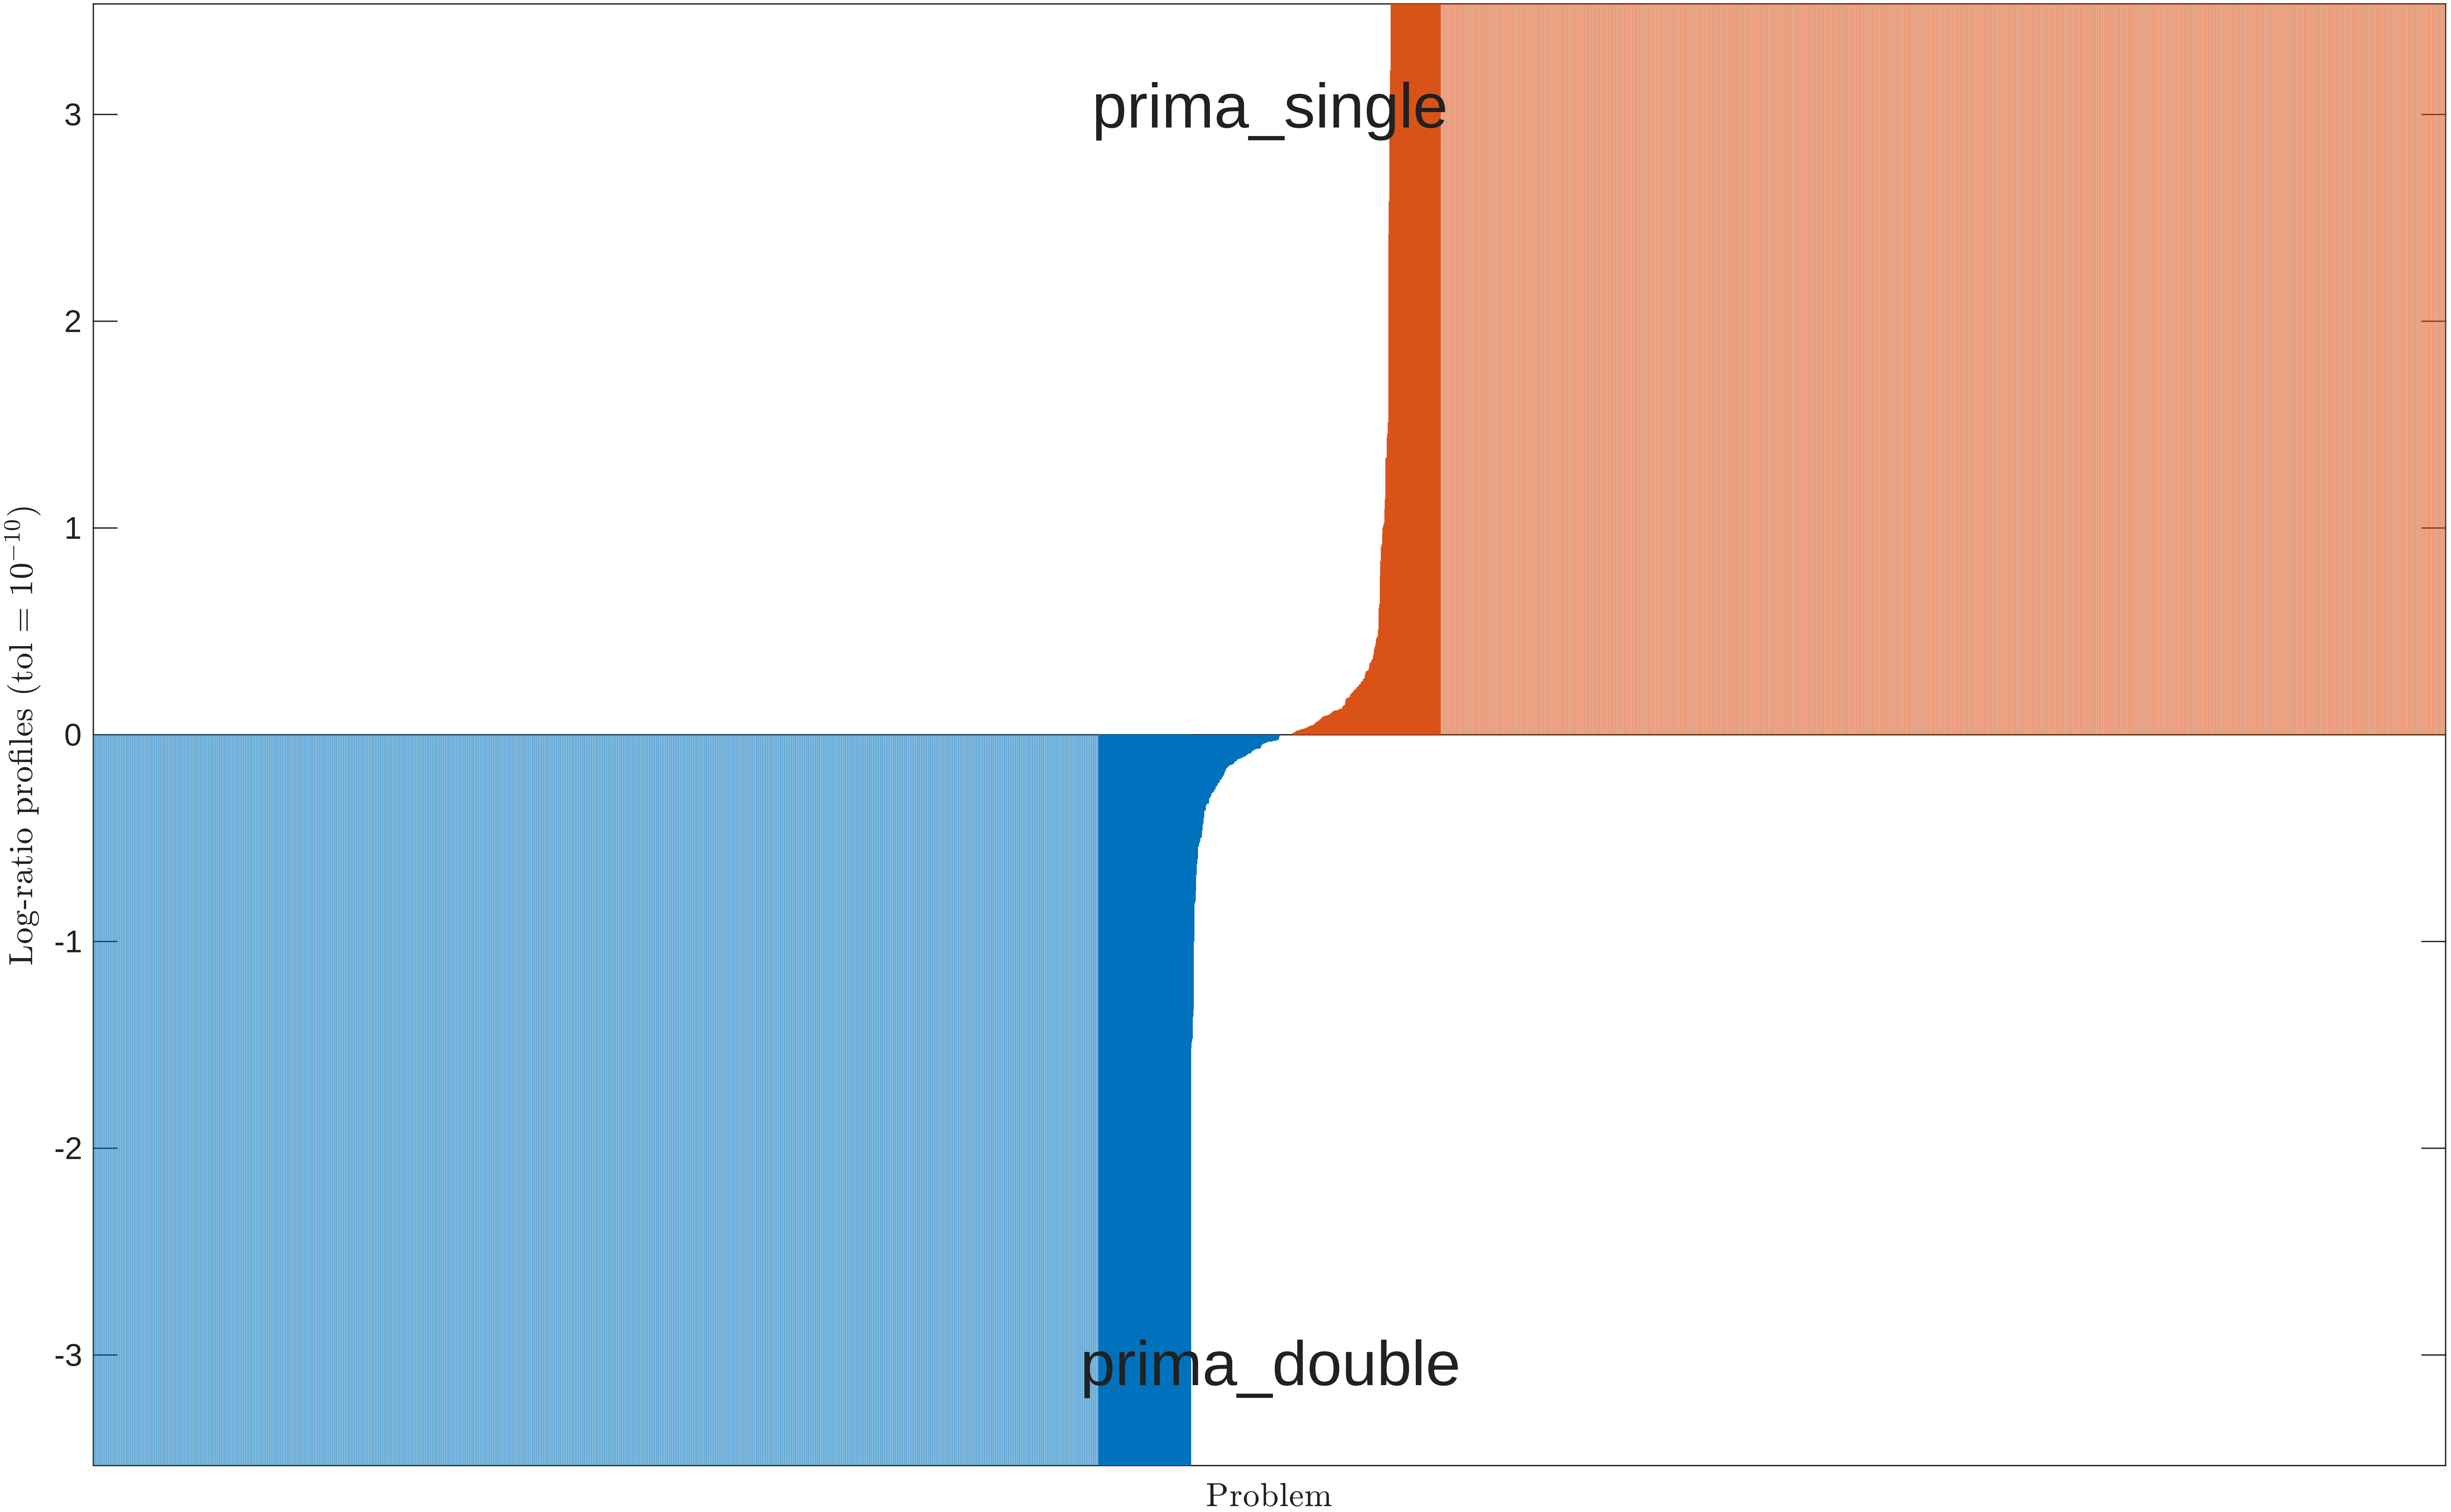
\includegraphics[width=0.75\textwidth]{figures/log_out_noisy_ds.png}
    \caption{Log-ratio profiles for double and single precision on the noisy problem set.}
    \label{fig:log_out_noisy_ds}
\end{figure}

The log‑ratio profiles reinforce this view. Whether examined problem by
problem or through aggregate scores, the conclusions remain the same.
More problems favor the double‑precision case over the single‑precision
one, especially at strict tolerances, while the gap shrinks under noise.
Between the double‑precision and quadruple‑precision cases, the
differences remain negligible throughout.

\ifnum\value{cite}>0
\small
\bibliography{ref.bib}
\bibliographystyle{plain}
\fi
\end{document}
